\documentclass[a4paper,12pt,oneside,openleft]{memoir}

% Castellano
\usepackage[english,spanish,es-tabla,es-noshorthands]{babel}
\selectlanguage{spanish}
\usepackage[utf8]{inputenc}
\usepackage[T1]{fontenc}
\usepackage{lmodern} % Scalable font
\usepackage{microtype}
\usepackage{placeins}

\RequirePackage{booktabs}
\RequirePackage[table]{xcolor}
\RequirePackage{xtab}
\RequirePackage{multirow}
\usepackage{tabularray}
\UseTblrLibrary{booktabs}

% Formatear números
\usepackage{siunitx}
\sisetup{
  output-decimal-marker = {,},   % coma para decimales
  group-separator       = {.},   % punto para los miles
  group-minimum-digits  = 4      % agrupa desde 4 cifras: 1.000
}

% Manejar acrónimos
\usepackage{acronym}

% Links
\PassOptionsToPackage{hyphens}{url}\usepackage[colorlinks]{hyperref}
\hypersetup{
	allcolors = {black}
}
\usepackage{csquotes}
\usepackage[backend=biber,style=numeric,sorting=none]{biblatex}
\setcounter{biburlnumpenalty}{9000}
\setcounter{biburlucpenalty}{9000}
\setcounter{biburllcpenalty}{9000}
\addbibresource{bibliografia.bib}

% Ecuaciones
\usepackage{amsmath}

% Rutas de fichero / paquete
\newcommand{\ruta}[1]{{\sffamily #1}}

% Párrafos
\nonzeroparskip

% Huérfanas y viudas
\widowpenalty100000
\clubpenalty100000

% Imágenes

% Comando para insertar una imagen en un lugar concreto.
% Los parámetros son:
% 1 --> Ruta absoluta/relativa de la figura
% 2 --> Texto a pie de figura
% 3 --> Tamaño en tanto por uno relativo al ancho de página
\usepackage{graphicx}
\newcommand{\imagen}[3]{
	\begin{figure}[!h]
		\centering
		\includegraphics[width=#3\textwidth]{#1}
		\caption{#2}\label{fig:#1}
	\end{figure}
	\FloatBarrier
}

% Comando para insertar una imagen sin posición.
% Los parámetros son:
% 1 --> Ruta absoluta/relativa de la figura
% 2 --> Texto a pie de figura
% 3 --> Tamaño en tanto por uno relativo al ancho de página
\newcommand{\imagenflotante}[3]{
	\begin{figure}
		\centering
		\includegraphics[width=#3\textwidth]{#1}
		\caption{#2}\label{fig:#1}
	\end{figure}
}

% El comando \figura nos permite insertar figuras comodamente, y utilizando
% siempre el mismo formato. Los parametros son:
% 1 --> Porcentaje del ancho de página que ocupará la figura (de 0 a 1)
% 2 --> Fichero de la imagen
% 3 --> Texto a pie de imagen
% 4 --> Etiqueta (label) para referencias
% 5 --> Opciones que queramos pasarle al \includegraphics
% 6 --> Opciones de posicionamiento a pasarle a \begin{figure}
\newcommand{\figuraConPosicion}[6]{%
  \setlength{\anchoFloat}{#1\textwidth}%
  \addtolength{\anchoFloat}{-4\fboxsep}%
  \setlength{\anchoFigura}{\anchoFloat}%
  \begin{figure}[#6]
    \begin{center}%
      \Ovalbox{%
        \begin{minipage}{\anchoFloat}%
          \begin{center}%
            \includegraphics[width=\anchoFigura,#5]{#2}%
            \caption{#3}%
            \label{#4}%
          \end{center}%
        \end{minipage}
      }%
    \end{center}%
  \end{figure}%
}

%
% Comando para incluir imágenes en formato apaisado (sin marco).
\newcommand{\figuraApaisadaSinMarco}[5]{%
  \begin{figure}%
    \begin{center}%
    \includegraphics[angle=90,height=#1\textheight,#5]{#2}%
    \caption{#3}%
    \label{#4}%
    \end{center}%
  \end{figure}%
}
% Para las tablas
\newcommand{\otoprule}{\midrule [\heavyrulewidth]}
%
% Nuevo comando para tablas pequeñas (menos de una página).
\newcommand{\tablaSmall}[5]{%
 \begin{table}
  \begin{center}
   \rowcolors {2}{gray!35}{}
   \begin{tabular}{#2}
    \toprule
    #4
    \otoprule
    #5
    \bottomrule
   \end{tabular}
   \caption{#1}
   \label{tabla:#3}
  \end{center}
 \end{table}
}

%
% Nuevo comando para tablas pequeñas (menos de una página).
\newcommand{\tablaSmallSinColores}[5]{%
 \begin{table}[H]
  \begin{center}
   \begin{tabular}{#2}
    \toprule
    #4
    \otoprule
    #5
    \bottomrule
   \end{tabular}
   \caption{#1}
   \label{tabla:#3}
  \end{center}
 \end{table}
}

\newcommand{\tablaApaisadaSmall}[5]{%
\begin{landscape}
  \begin{table}
   \begin{center}
    \rowcolors {2}{gray!35}{}
    \begin{tabular}{#2}
     \toprule
     #4
     \otoprule
     #5
     \bottomrule
    \end{tabular}
    \caption{#1}
    \label{tabla:#3}
   \end{center}
  \end{table}
\end{landscape}
}

%
% Nuevo comando para tablas grandes con cabecera y filas alternas coloreadas en gris.
\newcommand{\tabla}[6]{%
  \begin{center}
    \tablefirsthead{
      \toprule
      #5
      \otoprule
    }
    \tablehead{
      \multicolumn{#3}{l}{\small\sl continúa desde la página anterior}\\
      \toprule
      #5
      \otoprule
    }
    \tabletail{
      \hline
      \multicolumn{#3}{r}{\small\sl continúa en la página siguiente}\\
    }
    \tablelasttail{
      \hline
    }
    \bottomcaption{#1}
    \rowcolors {2}{gray!35}{}
    \begin{xtabular}{#2}
      #6
      \bottomrule
    \end{xtabular}
    \label{tabla:#4}
  \end{center}
}

%
% Nuevo comando para tablas grandes con cabecera.
\newcommand{\tablaSinColores}[6]{%
  \begin{center}
    \tablefirsthead{
      \toprule
      #5
      \otoprule
    }
    \tablehead{
      \multicolumn{#3}{l}{\small\sl continúa desde la página anterior}\\
      \toprule
      #5
      \otoprule
    }
    \tabletail{
      \hline
      \multicolumn{#3}{r}{\small\sl continúa en la página siguiente}\\
    }
    \tablelasttail{
      \hline
    }
    \bottomcaption{#1}
    \begin{xtabular}{#2}
      #6
      \bottomrule
    \end{xtabular}
    \label{tabla:#4}
  \end{center}
}

%
% Nuevo comando para tablas grandes sin cabecera.
\newcommand{\tablaSinCabecera}[5]{%
  \begin{center}
    \tablefirsthead{
      \toprule
    }
    \tablehead{
      \multicolumn{#3}{l}{\small\sl continúa desde la página anterior}\\
      \hline
    }
    \tabletail{
      \hline
      \multicolumn{#3}{r}{\small\sl continúa en la página siguiente}\\
    }
    \tablelasttail{
      \hline
    }
    \bottomcaption{#1}
  \begin{xtabular}{#2}
    #5
   \bottomrule
  \end{xtabular}
  \label{tabla:#4}
  \end{center}
}



\definecolor{cgoLight}{HTML}{EEEEEE}
\definecolor{cgoExtralight}{HTML}{FFFFFF}

%
% Nuevo comando para tablas grandes sin cabecera.
\newcommand{\tablaSinCabeceraConBandas}[5]{%
  \begin{center}
    \tablefirsthead{
      \toprule
    }
    \tablehead{
      \multicolumn{#3}{l}{\small\sl continúa desde la página anterior}\\
      \hline
    }
    \tabletail{
      \hline
      \multicolumn{#3}{r}{\small\sl continúa en la página siguiente}\\
    }
    \tablelasttail{
      \hline
    }
    \bottomcaption{#1}
    \rowcolors[]{1}{cgoExtralight}{cgoLight}

  \begin{xtabular}{#2}
    #5
   \bottomrule
  \end{xtabular}
  \label{tabla:#4}
  \end{center}
}



\graphicspath{ {./img/} }

% Capítulos
\chapterstyle{bianchi}
\newcommand{\capitulo}[2]{
	\setcounter{chapter}{#1}
	\setcounter{section}{0}
	\setcounter{figure}{0}
	\setcounter{table}{0}
	\chapter*{\thechapter.\enskip #2}
	\addcontentsline{toc}{chapter}{\thechapter.\enskip #2}
	\markboth{#2}{#2}
}

% Apéndices
\renewcommand{\appendixname}{Apéndice}
\renewcommand*\cftappendixname{\appendixname}

\newcommand{\apendice}[1]{
	%\renewcommand{\thechapter}{A}
	\chapter{#1}
}

\renewcommand*\cftappendixname{\appendixname\ }

% Formato de portada
\makeatletter
\newcommand{\tutor}[1]{\def\@tutor{#1}}
\newcommand{\course}[1]{\def\@course{#1}}
\definecolor{cpardoBox}{HTML}{E6E6FF}
\def\maketitle{
  \null
  \thispagestyle{empty}
  % Cabecera ----------------
\noindent
\includegraphics[width=\textwidth]{institucional/cabecera}\vspace{1cm}%
  \vfill
  % Título proyecto y escudo informática ----------------
  \colorbox{cpardoBox}{%
    \begin{minipage}{.8\textwidth}
      \vspace{.5cm}\Large
      \begin{center}
      \textbf{TFG del Grado en Ingeniería Informática}\vspace{.6cm}\\
      \textbf{\LARGE\@title{}}
      \end{center}
      \vspace{.2cm}
    \end{minipage}

  }%
  \hfill\begin{minipage}{.20\textwidth}
    
\includegraphics[width=\textwidth]{institucional/escudo-informatica}
  \end{minipage}
  \vfill
  % Datos de alumno, curso y tutores ------------------
  \begin{center}%
  {%
    \noindent\LARGE
    Presentado por \@author{}\\
    en Universidad de Burgos\\
    \@date{}\\
    Tutor: \@tutor{}\\[.6em]
    Cotutores empresariales:\\[.2em]
    \tutoresEmpresariales\\
  }%
  \end{center}%
  \null
  \cleardoublepage
  }
\makeatother

% Se definen los datos generales del documento.
\newcommand{\titulo}{Manualito}
\newcommand{\subtitulo}{Aplicación web de apoyo al aprendizaje de juegos de mesa}
\newcommand{\nombre}{Ibai Moya Aroz}
\newcommand{\dni}{DNI CENSORED}
\newcommand{\nombreTutor}{Bruno Baruque Zanón}
\newcommand{\tutoresEmpresariales}{Pablo García Ullán,\\Luis Peralta\\y Ánder Bermúdez González}
\newcommand{\departamentoTutor}{Departamento de Ingeniería Informática}
\newcommand{\areaTutor}{Área de Lenguajes y Sistemas Informáticos}
\newcommand{\fechaEntrega}{17 de septiembre de 2026}
\newcommand{\nombreGrado}{Grado en Ingeniería Informática}
\newcommand{\ciudad}{Burgos}
\newcommand{\nombreUniversidad}{Universidad de \ciudad}


% Datos de portada.
\title{{\Huge \titulo}\\[0.5cm]\subtitulo}
\author{\nombre}
\tutor{\nombreTutor}
\date{\fechaEntrega}


\begin{document}

\maketitle


\newpage\null\thispagestyle{empty}\newpage


%%%%%%%%%%%%%%%%%%%%%%%%%%%%%%%%%%%%%%%%%%%%%%%%%%%%%%%%%%%%%%%%%%%%%%%%%%%%%%%%%%%%%%%%
\thispagestyle{empty}


\noindent
\includegraphics[width=\textwidth]{institucional/cabecera}\vspace{1cm}

\noindent D. \nombreTutor, profesor del \departamentoTutor, \areaTutor.

\noindent Expone:

\noindent Que el alumno D. \nombre, con \dni, ha realizado el Trabajo final de Grado en Ingeniería Informática titulado \textit{\titulo: \subtitulo}.

\noindent Y que dicho trabajo ha sido realizado por el alumno bajo la dirección del que suscribe, en virtud de lo cual se autoriza su presentación y defensa.

\begin{center} %\large
En \ciudad, {\large \fechaEntrega}
\end{center}

\vfill\vfill\vfill

\begin{center}
Vº. Bº. del Tutor:\\[2cm]
D. Bruno Baruque Zanón
\end{center}


\newpage\null\thispagestyle{empty}\newpage




\frontmatter

% Abstract en castellano
\renewcommand*\abstractname{Resumen}
\begin{abstract}
Aprender un juego de mesa puede requerir una lectura extensa de su manual,
a su vez, resolver una duda durante la partida obliga a localizar la
regla correspondiente. Para facilitar ambas tareas, se ha desarrollado
\textit{Manualito}, una aplicación web que permite obtener de forma ágil una
explicación general del juego y plantear preguntas a un asistente de
inteligencia artificial.

La aplicación extrae el texto de manuales en archivos \acs{PDF} o imágenes,
utilizando reconocimiento óptico de caracteres cuando es necesario, y
permite revisarlo junto a las páginas originales. A partir de ese contenido,
combina la búsqueda por palabras y por significado para seleccionar la
información que reciben los modelos de lenguaje ejecutados localmente.
Este enfoque de generación aumentada por recuperación busca reducir el
riesgo de que el asistente invente reglas, mientras que las referencias a
las páginas consultadas permiten comprobar sus respuestas.

Durante el desarrollo se compararon alternativas de reconocimiento de
texto, recuperación y modelos de lenguaje para ajustar el sistema a los
recursos disponibles. El resultado reúne estas funciones con la gestión de
juegos, manuales y conversaciones, de modo que el usuario puede conservar
la información y retomarla en futuras partidas.
\end{abstract}

\renewcommand*\abstractname{Descriptores}
\begin{abstract}
Juegos de mesa, aplicación web, reconocimiento óptico de caracteres, modelos
de lenguaje, generación aumentada por recuperación, inteligencia artificial,
procesamiento del lenguaje natural, recuperación de información, búsqueda
híbrida, consulta de reglas.
\end{abstract}

\clearpage

% Abstract en inglés
\begin{otherlanguage}{english}
\renewcommand*\abstractname{Abstract}
\begin{abstract}
Learning a board game can require extensive reading of its rulebook,
in addition, resolving a question during play means finding the relevant rule.
To support both tasks, \textit{Manualito} was developed as a web application
that lets users quickly obtain an overview of a game and ask an artificial
intelligence assistant questions about it.

The application extracts text from rulebooks supplied as \acs{PDF} files or
images, using optical character recognition when necessary, and allows
users to review it alongside the original pages. It then combines keyword
and semantic search to select the information provided to locally run
language models. This retrieval-augmented generation approach aims to
reduce the risk of the assistant inventing rules, while references to the
source pages allow users to check its answers.

During development, alternatives for text recognition, retrieval and
language models were compared to adapt the system to the available
resources. The resulting application combines these functions with the
management of games, rulebooks and conversations, allowing users to save
the information and return to it in future game sessions.
\end{abstract}

\renewcommand*\abstractname{Keywords}
\begin{abstract}
Board games, web application, optical character recognition, language models,
retrieval-augmented generation, artificial intelligence, natural language
processing, information retrieval, hybrid search, rule consultation.
\end{abstract}
\end{otherlanguage}

\clearpage

% Indices
\tableofcontents

\clearpage

\listoffigures

\clearpage

\listoftables

\clearpage
\chapter*{Lista de acrónimos}
\addcontentsline{toc}{chapter}{Lista de acrónimos}
\begin{acronym}[WWWWW] % plantilla de la sigla más ancha, para alinear
    \acro{BM25}{\textit{Best Match 25}}
    \acro{CD}{\textit{Continuous Deployment}}
    \acro{CI}{\textit{Continuous Integration}}
    \acro{CPU}{\textit{Central Processing Unit}}
    \acro{CSRF}{\textit{Cross-Site Request Forgery}}
    \acro{GPU}{\textit{Graphics Processing Unit}}
    \acro{HNSW}{\textit{Hierarchical Navigable Small World}}
    \acro{LLM}{\textit{Large Language Model}}
    \acro{ML}{\textit{Machine Learning}}
    \acro{OCR}{\textit{Optical Character Recognition}}
    \acro{PDF}{\textit{Portable Document Format}}
    \acro{RAG}{\textit{Retrieval-Augmented Generation}}
    \acro{ReDoS}{\textit{Regular Expression Denial of Service}}
    \acro{RRF}{\textit{Reciprocal Rank Fusion}}
    \acro{TDD}{\textit{Test-Driven Development}}
    \acro{TTS}{\textit{Text-To-Speech}}
    \acro{XSS}{\textit{Cross-Site Scripting}}
\end{acronym}

\clearpage

\mainmatter
\capitulo{1}{Introducción}

En ocasiones, ya sea en familia, con amigos o en solitario, tenemos ganas de
probar un juego de mesa nuevo. Sin embargo, nos echamos atrás al ver la
cantidad de reglas e instrucciones que hay que leer y entender antes de
empezar a jugar.

Además, haber leído el manual no significa que hayamos comprendido todas las
reglas. Durante una partida pueden aparecer dudas sobre una acción, una
excepción o una situación que no habíamos previsto. Para resolverlas, hay que
volver al reglamento y buscar la explicación que corresponde a ese
caso en concreto.

Para ayudar en estas situaciones, se ha desarrollado \textit{Manualito},
una aplicación web que permite obtener de forma ágil una explicación
general de un juego de mesa y plantear dudas sobre sus reglas a un
asistente de inteligencia artificial que se encarga de consultar los
manuales para resolverlas.

En su estudio sobre el uso de herramientas digitales en juegos de mesa,
Rogerson y sus colaboradores destacan la importancia de integrarlas en la
experiencia de juego sin que se conviertan en una distracción
~\cite{rogerson2021gimmick}. En esta línea,
\textit{Manualito} se plantea como una herramienta de apoyo a la que
acudir cuando surge una duda sobre las reglas durante la partida.

Para utilizar la aplicación, el usuario puede añadir los manuales en archivos
\acs{PDF} o imágenes y asociarlos al juego correspondiente. A partir de
ellos se extrae el texto, utilizando reconocimiento óptico de caracteres,
denominado \acs{OCR}, cuando es necesario.\acused{OCR} El texto obtenido se
puede revisar junto a las páginas originales y corregir si contiene errores.
Los manuales y las conversaciones se guardan para poder volver a consultarlos
en otra partida.

Las respuestas se generan con un modelo de lenguaje al que se proporciona
información de los manuales. Para encontrar los pasajes relacionados con una
pregunta se utiliza generación aumentada por recuperación, conocida como
\acs{RAG} por \emph{Retrieval-Augmented Generation}~\cite{lewis2020rag}.\acused{RAG}
La búsqueda se limita a los manuales del juego a los que el usuario tiene
acceso. Los fragmentos encontrados se envían al modelo como contexto y la
respuesta se muestra junto a referencias a las páginas recuperadas, para que
el usuario pueda consultar su contenido.

Toda esta estructura busca reducir el riesgo de alucinaciones, es decir,
de que el asistente invente reglas o detalles al
responder~\cite{kalai2025hallucinate}. Para ello, el modelo recibe
información de los manuales relacionada con la pregunta del usuario.
La posibilidad de corregir el texto extraído y consultar las páginas
originales permite, además, detectar errores y comprobar las
explicaciones en su contexto.

Aunque \textit{Manualito} se centra en explicar juegos de mesa, el mismo enfoque
podría adaptarse a otros ámbitos en los que sea necesario consultar manuales
o seguir procedimientos. Un ejemplo sería la consulta de protocolos de
actuación ante un incidente de ciberseguridad, donde puede ser necesario
combinar instrucciones de análisis, recuperación de sistemas y protección
de datos. Los juegos de mesa sirven así como caso de estudio, mientras que
su aplicación en otros contextos requeriría adaptar el sistema y evaluar
sus respuestas.

\section{Materiales del proyecto}
\label{intro:materiales}

La aplicación, el código fuente, la documentación y los materiales de
evaluación del proyecto se encuentran en los siguientes recursos:

\begin{itemize}
    \item \textbf{Sitio web del proyecto.}
    Presenta \textit{Manualito} y sirve como punto de entrada en
    \url{https://manualito.dev/}.

    \item \textbf{Aplicación web.}
    La versión desplegada puede consultarse en
    \url{https://app.manualito.dev/}.

    \item \textbf{Repositorio de GitHub.}
    Incluye la aplicación y los archivos necesarios para preparar y ejecutar
    el entorno en \url{https://github.com/ibaimoya/manualito}
    ~\cite{manualito_repositorio}.

    \item \textbf{Repositorio de GitLab.}
    Conserva la copia de desarrollo del proyecto. Puede consultarse en
    \href{https://gitlab.com/HP-SCDS/Observatorio/2025-2026/manualito/ubu-manualito}
    {\url{gitlab.com/HP-SCDS/Observatorio/2025-2026/manualito/ubu-manualito}}
    ~\cite{manualito_gitlab}.

    \item \textbf{Documentación web.}
    Reúne las guías de uso y la documentación técnica del proyecto.
    Puede consultarse en \url{https://docs.manualito.dev/}
    ~\cite{manualito_documentacion}.

    \item \textbf{Benchmarks.}
    Los \textit{notebooks} y resultados de las pruebas se pueden consultar en el
    directorio \href{https://github.com/ibaimoya/manualito/tree/master/docs/benchmarks}
    {\texttt{docs/benchmarks}} del repositorio de GitHub~\cite{manualito_benchmarks}.
\end{itemize}

\capitulo{2}{Objetivos del proyecto}

A continuación, se detallan todos los objetivos que se persiguen con
el desarrollo de \textit{Manualito}.

\section{Objetivos generales}
\label{objetivos:generales}

El proyecto persigue los siguientes objetivos generales, que se desarrollan
en la especificación de requisitos del Anexo B:

\begin{itemize}
    \item Desarrollar una aplicación web que facilite el
    aprendizaje y la consulta de las instrucciones y reglas de juegos de mesa.

    \item Procesar manuales en distintos formatos para extraer
    su contenido y utilizarlo dentro de la aplicación.

    \item Generar explicaciones y responder preguntas sobre
    un juego a partir de la información contenida en sus manuales.

    \item Almacenar de forma organizada la información de los
    juegos, los manuales y las conversaciones de cada usuario para permitir
    su consulta posterior.

    \item Proteger las cuentas y la información de los
    usuarios frente a accesos y modificaciones sin permiso.
\end{itemize}

\section{Objetivos técnicos}
\label{objetivos:especificos}

Se plantean los siguientes objetivos técnicos:

\begin{itemize}
    \item Integrar técnicas de \acs{OCR} para extraer y preparar el texto
    de los manuales.

    \item Diseñar un sistema \acs{RAG} que combine búsqueda léxica y
    semántica para fundamentar las respuestas del modelo.

    \item Integrar modelos de lenguaje ejecutados localmente mediante
    Ollama.

    \item Desarrollar la interfaz con React y TypeScript y el servidor
    con FastAPI.

    \item Aplicar una arquitectura modular y patrones de diseño que
    faciliten el mantenimiento.

    \item Utilizar PostgreSQL para la persistencia y ChromaDB para la
    búsqueda vectorial.

    \item Gestionar las tareas de procesamiento en segundo plano
    mediante Celery y Redis.

    \item Preparar un despliegue reproducible mediante Docker Compose
    y gestionar la infraestructura con Terraform.

    \item Utilizar Git con GitHub y GitLab para el control de versiones.

    \item Automatizar las pruebas y el análisis de calidad mediante
    integración continua, y publicar la parte estática mediante
    despliegue continuo.

    \item Evaluar las distintas tecnologías del
    sistema mediante pruebas de rendimiento.
\end{itemize}

\section{Objetivos personales}
\label{objetivos:personales}

Además de mencionar los objetivos generales y técnicos, se
presentan los objetivos a nivel personal que me han llevado a
desarrollar este proyecto:

\begin{itemize}
    \item Adquirir conocimientos de tecnologías y arquitecturas
    del campo de la inteligencia artificial.

    \item Comprender el ciclo de desarrollo y despliegue de una
    aplicación web.

    \item Mejorar la capacidad para planificar y organizar un
    proyecto de desarrollo.

    \item Profundizar en el diseño y desarrollo de interfaces de usuario.

    \item Explorar el desarrollo agéntico~\cite{ibm_agentic_coding}
    como apoyo en tareas concretas del proyecto.
\end{itemize}

\capitulo{3}{Conceptos teóricos}

Una pregunta sobre una regla durante una partida de un juego de mesa normalmente depende de una regla algo general, sin embargo, en ocasiones puede depender a su vez de una excepción que aparece varias páginas después. Por tanto, para responder correctamente a dicha pregunta a partir del reglamento, primero hay que obtener su texto y localizar los pasajes que permiten resolver la pregunta. Sobre esta información se puede crear una explicación, conservando la relación con las páginas de origen.

Este proceso se trata del núcleo técnico de este proyecto y, se realiza utilizando los conceptos que se detallan a continuación, desde el reconocimiento del texto hasta la búsqueda y la generación de respuestas
mediante un \ac{LLM}.

\section{Extracción y reconocimiento de texto}

Aunque dos páginas de un archivo \acs{PDF} tengan el mismo aspecto, su
contenido puede estar almacenado de forma distinta. Un documento creado
digitalmente suele conservar los caracteres, por lo que es posible extraerlos
directamente, mientras que una página escaneada puede contener únicamente una
imagen. Además, la disposición visual del documento no siempre se traslada al
texto extraído, especialmente cuando hay columnas, tablas o elementos
superpuestos~\cite{pypdf_extraccion}.

Cuando el texto solo está disponible como imagen, se recurre al
reconocimiento óptico de caracteres, \acs{OCR}. Esta técnica permite localizar
las zonas que contienen escritura y reconocer los caracteres que aparecen en
ellas, de modo que el texto pueda buscarse y procesarse. El resultado depende
tanto del reconocimiento como de la calidad de la imagen de
entrada~\cite{tesseract_calidad}.

Los ejemplos de esta sección utilizan una fotografía del manual de Monopoly
de Jose Antonio Ortigueira Amor~\cite{ortigueira_monopoly_2022}, publicada bajo
la licencia \href{https://creativecommons.org/licenses/by/4.0/}{Creative Commons
Reconocimiento 4.0}. En la figura~\ref{fig:ocr-original} se han añadido una
ampliación y marcas para señalar las dificultades del documento, donde aparecen
dos páginas juntas y los pliegues del papel atraviesan algunas líneas.
La iluminación tampoco es
uniforme, por lo que no todas las letras se distinguen igual del fondo.
Estas dificultades ayudan a entender por qué obtener el texto no consiste
únicamente en identificar caracteres aislados.

\begin{figure}[htbp]
    \centering
    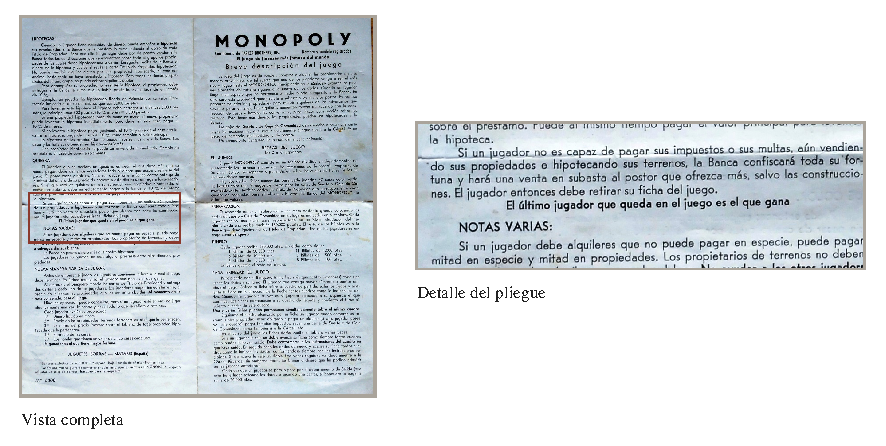
\includegraphics[width=\textwidth]{memoria/conceptos-teoricos/ejemplo-ocr/original-detalle.pdf}
    \caption{Fotografía de un manual con dificultades para el reconocimiento}
    \label{fig:ocr-original}
\end{figure}

\FloatBarrier

\subsection{Preprocesado de la imagen}

Antes del reconocimiento se puede ajustar la escala, reducir el ruido,
corregir la inclinación o separar el texto del fondo mediante una imagen en
blanco y negro. Estas operaciones buscan que los caracteres sean más fáciles
de distinguir, aunque su utilidad depende del documento. En una fotografía
como la anterior, las diferencias de iluminación pueden hacer que un mismo
ajuste aclare una zona y oculte parte del texto en otra. Por ello, no todos
los documentos necesitan el mismo tratamiento ni aplicar más ajustes implica
obtener un mejor resultado~\cite{tesseract_calidad}.

La figura~\ref{fig:ocr-preprocesado} muestra un fragmento de esa fotografía
después de aplicar los preprocesados utilizados en Manualito. Para Tesseract se amplía
la imagen por un factor de 2,5 y se convierte a escala de grises, mientras
que para PaddleOCR se trabaja también en escala de grises y se ajusta el
contraste por zonas. Este último tratamiento permite adaptar el contraste
a las diferencias de iluminación dentro de una misma
imagen~\cite{opencv_contraste}.

Los tratamientos se han aplicado a la fotografía completa antes de recortar
el fragmento. Los tres recuadros tienen el mismo tamaño y están centrados
en el mismo punto de la fotografía. El de Tesseract muestra una zona menor,
con el texto ampliado por un factor de 2,5, mientras que el original y el de
PaddleOCR conservan el mismo encuadre. La figura permite observar los cambios
en la imagen, pero no demuestra
por sí sola una mejora en el reconocimiento del texto.

\begin{figure}[htbp]
    \centering
    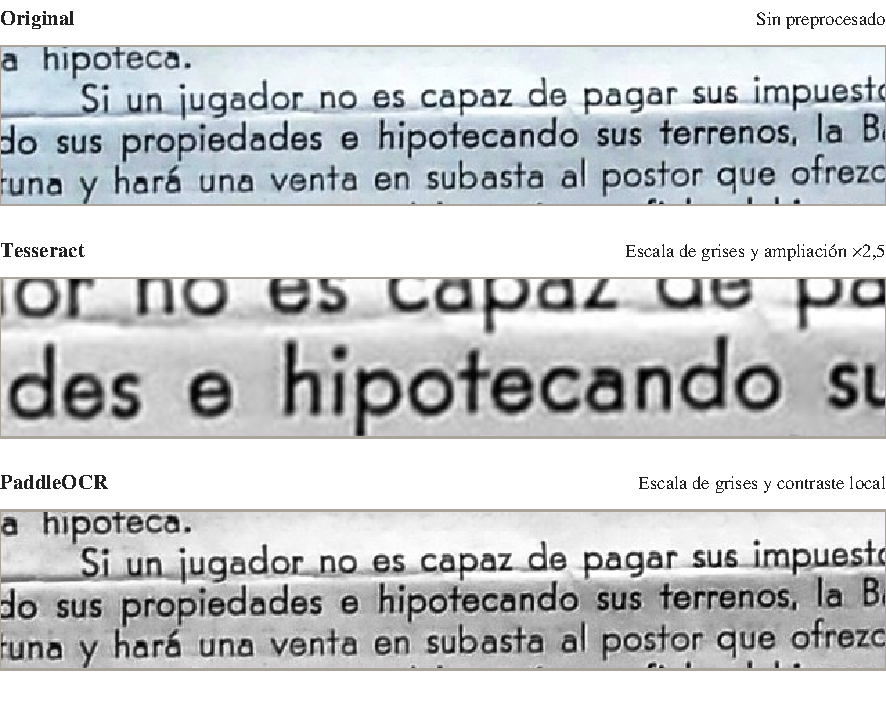
\includegraphics[width=\textwidth]{memoria/conceptos-teoricos/ejemplo-ocr/comparacion-preprocesado.pdf}
    \caption{Preprocesado de la imagen para Tesseract y PaddleOCR}
    \label{fig:ocr-preprocesado}
\end{figure}

\FloatBarrier

\subsection{Reconocimiento y orden de lectura}

Localizar el texto y reconocerlo son tareas distintas. La primera determina
qué zonas de la imagen contienen escritura, mientras que la segunda obtiene
los caracteres que aparecen en ellas. Las zonas pueden representarse mediante
recuadros, conocidos como \textit{bounding boxes}, que sitúan bloques, líneas
o palabras dentro de la página~\cite{tesseract_salida_ocr}.

Reconocer correctamente las palabras no es suficiente. También hay que
conservar el orden de lectura, que resulta más fácil de seguir en un párrafo
continuo que en una página con varias columnas o imágenes intercaladas.
Si se toma una línea de cada columna de forma alterna, pueden mezclarse
fragmentos que pertenecen a explicaciones distintas. Esta dificultad no se
limita al \acs{OCR}, también puede aparecer al extraer los caracteres de un
\acs{PDF} creado digitalmente~\cite{pypdf_extraccion,tesseract_calidad}.

La figura~\ref{fig:ocr-reconocimiento} ilustra este problema con dos recortes
de la fotografía del manual de Monopoly. Las transcripciones se han abreviado
y distribuido manualmente para el ejemplo, por lo que no representan la salida
de un motor de \acs{OCR}. Si se lee cada bloque por separado, se conserva el
sentido de ambos textos, mientras que al unir una línea de la izquierda con
otra de la derecha se mezclan la explicación de las hipotecas y la descripción
del juego. Aunque las palabras son las mismas, el resultado deja de tener sentido.
En este manual, además, la presentación del juego está a la derecha y los
apartados posteriores a la izquierda.

\begin{figure}[htbp]
    \centering
    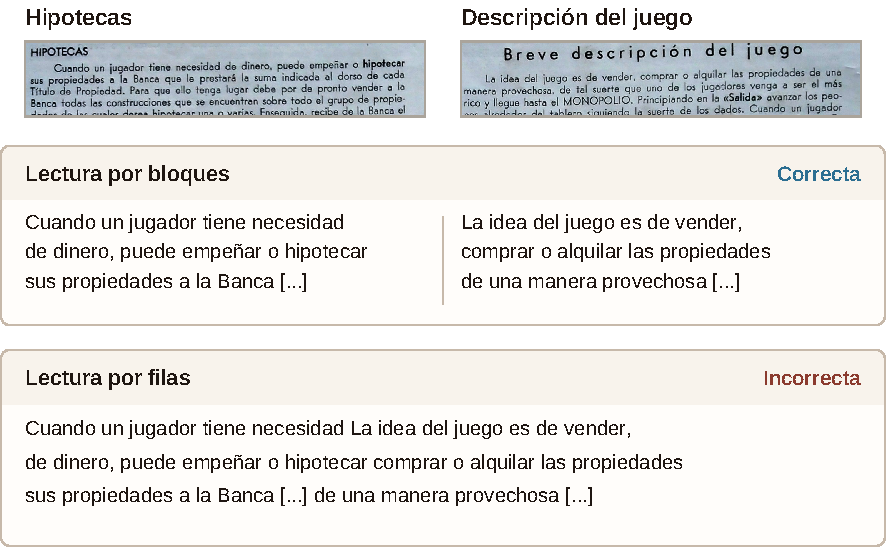
\includegraphics[width=\textwidth]{memoria/conceptos-teoricos/ejemplo-ocr/orden-columnas.pdf}
    \caption{Lectura por bloques y por filas}
    \label{fig:ocr-reconocimiento}
\end{figure}

\FloatBarrier

\subsection{Posprocesado del texto}

Una vez reconocido el texto, se puede revisar su formato para corregir
espacios duplicados, saltos de línea o palabras partidas entre dos líneas.
Esta limpieza no debe confundirse con modificar el contenido. En un
reglamento, cambiar una cifra o eliminar una negación puede alterar por
completo una regla, de modo que cualquier corrección debe conservar su
significado y permitir contrastar el resultado con la página original.

La figura~\ref{fig:ocr-posprocesado} muestra ejemplos obtenidos en una ejecución
local al procesar la fotografía de Monopoly con Tesseract 5.4.0 y aplicar las
reglas de Manualito. Los fragmentos conservan los saltos de línea reconocidos
y permiten ver cómo las palabras partidas por un guion se unen cuando la
palabra resultante pertenece al vocabulario utilizado, mientras que algunas
líneas breves con baja confianza se filtran porque pueden ser ruido. En esta
prueba se han aplicado únicamente la limpieza y las reglas, sin corrección
mediante un modelo de lenguaje.

\begin{figure}[htbp]
    \centering
    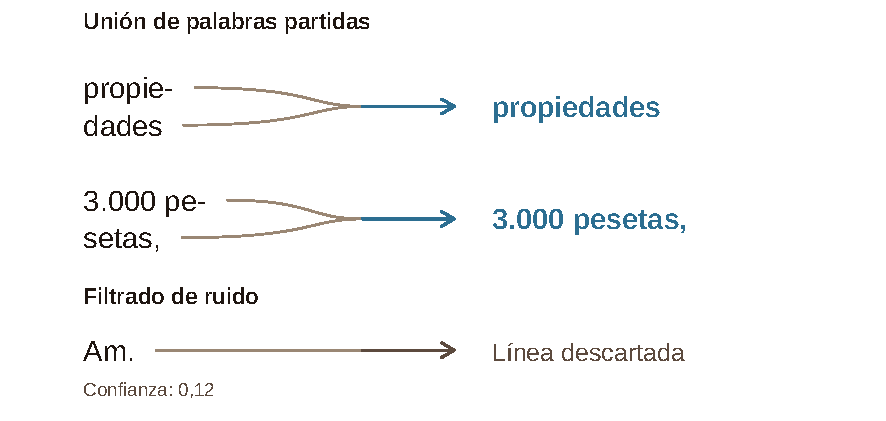
\includegraphics[width=\textwidth]{memoria/conceptos-teoricos/ejemplo-ocr/posprocesado-tabla.pdf}
    \caption{Ejemplos de posprocesado del texto de Monopoly}
    \label{fig:ocr-posprocesado}
\end{figure}

\FloatBarrier

Además del texto, un motor de \acs{OCR} puede proporcionar una puntuación de
confianza asociada al reconocimiento~\cite{tesseract_salida_ocr}. Este valor
no indica que las reglas se hayan interpretado bien, ya que una transcripción
legible también puede contener errores que cambien su significado. En esta
misma prueba, una línea con confianza superior a 0,90 contiene \enquote{10 Y}
en lugar de \enquote{10 \%}. Las reglas aplicadas no corrigen ese error, por lo
que sigue siendo necesario poder revisar el texto junto a la imagen original.

\section{Modelos de lenguaje}

Los grandes modelos de lenguaje, \acs{LLM}\acused{LLM}, son redes neuronales
entrenadas con grandes cantidades de texto para aprender relaciones entre sus
elementos. En los modelos generativos autorregresivos, la respuesta se
construye añadiendo una unidad de texto tras otra, según las probabilidades que
el modelo asigna a las posibles continuaciones del texto anterior. Este uso del
modelo ya entrenado se denomina \textit{inferencia} y permite realizar
distintas tareas a partir de instrucciones y ejemplos~\cite{brown2020language}.

Al analizar este funcionamiento, Bender et al. introducen la metáfora de los
\enquote{loros estocásticos} para advertir de que generar texto fluido a partir
de patrones estadísticos no implica, por sí solo, comprender su
significado~\cite{bender2021stochastic}.

\subsection{\textit{Tokens}, instrucciones y contexto}

Antes de procesar el texto, el proceso de \textit{tokenización} lo divide en
unidades llamadas \textit{tokens}, que se representan mediante
identificadores numéricos. Un \textit{token} puede corresponder a una
palabra, parte de ella o incluso a signos de puntuación. La división depende
de un componente llamado \textit{tokenizador}, por lo que dos modelos pueden
representar la misma frase con un número diferente de
\textit{tokens}~\cite{hf_tokenizacion}.

El texto que se proporciona al modelo para indicarle qué debe generar recibe
el nombre de \textit{prompt}. Puede contener las instrucciones de la tarea, la
pregunta, ejemplos y el contenido necesario para responder~\cite{brown2020language}.
Por ejemplo, si se pregunta cómo se mueve una torre en ajedrez, el
\textit{prompt} puede incluir la regla de movimiento y pedir al modelo que la
utilice para explicarlo. También se puede indicar que la respuesta sea
breve o que incluya un ejemplo, según la explicación que se quiera obtener.

La \textit{ventana de contexto} establece cuántos \textit{tokens} puede manejar el
modelo en una ejecución~\cite{ollama_contexto}. Por ello, al preparar una
consulta hay que distribuir ese espacio entre las instrucciones, el historial,
el contenido de referencia y la respuesta que se espera generar. Un historial
cada vez más largo deja menos espacio para los pasajes del manual, de modo que
es necesario seleccionar la información que se envía al modelo.

Durante la generación, también se puede ajustar el cómo se elige el siguiente
\textit{token}. Por ejemplo, la \textit{temperatura} modifica la distribución de
probabilidades utilizada en el muestreo. Un valor más pequeño concentra la
elección en las opciones más probables, pero no garantiza que la respuesta sea correcta~\cite{hf_generacion}.

\subsection{Cuantización}

Los parámetros aprendidos por un modelo se almacenan como valores numéricos y
ocupan memoria. La \textit{cuantización} permite representarlos con menos bits,
por ejemplo, pasando de una representación de 16 bits a otra de 8 o de 4 bits.
De este modo, se logra reducir el espacio necesario para almacenarlos, a cambio
de introducir una aproximación que puede afectar a la calidad del
modelo~\cite{hf_cuantizacion}.

Esta reducción resulta útil cuando se dispone de recursos limitados, pero el
ahorro en los parámetros no representa todo el consumo durante la ejecución,
que también incluye estructuras que conservan información de los \textit{tokens} ya
procesados~\cite{hf_cache}. Cuantizar cambia la representación de esos valores,
mientras que ajustar la temperatura modifica la selección del siguiente \textit{token}.
Estas operaciones son algo distinto al \textit{ajuste fino} o \textit{fine-
tuning}, que consiste en continuar el entrenamiento con el objetivo de adaptar
el modelo a una tarea~\cite{hf_ajuste_fino}.

\subsection{Alucinaciones}

Las alucinaciones son respuestas que presentan información falsa o sin
fundamento como si fuera cierta. Kalai et al. analizan por qué pueden aparecer
incluso cuando los datos de entrenamiento no contienen errores, así como el
papel de las evaluaciones que favorecen responder antes que reconocer la
incertidumbre~\cite{kalai2025hallucinate}.

Al explicar el movimiento del alfil, el modelo podría afirmar que puede
saltar otras piezas, aunque las reglas no lo
permiten~\cite{fide2023ajedrez}. Para reducir este tipo de errores, la generación puede apoyarse en pasajes recuperados del
documento y en instrucciones que limiten la respuesta a esa información. Este
es el punto de partida de la generación aumentada por
recuperación~\cite{lewis2020rag}.

\section{Generación aumentada por recuperación}

La generación aumentada por recuperación, \acs{RAG}, combina la búsqueda de
información externa con un modelo generativo. Ante una pregunta, se seleccionan
documentos o pasajes relevantes y se incorporan a la entrada del modelo para
que pueda basar su respuesta en ellos. De esta manera, la información
disponible se ve enriquecida y no se limita a la que quedó recogida en sus
parámetros durante el entrenamiento~\cite{lewis2020rag}.

La figura~\ref{fig:teoria-rag} ilustra este proceso con dos páginas creadas
para el ejemplo a partir de una síntesis de las reglas de
ajedrez~\cite{fide2023ajedrez}. Ante la pregunta sobre el avance del peón, se recuperan los
pasajes que explican su primer movimiento y las condiciones para realizarlo.
El modelo recibe esos pasajes junto con la pregunta para preparar la respuesta,
que conserva la referencia a la página consultada.

\begin{figure}[htbp]
    \centering
    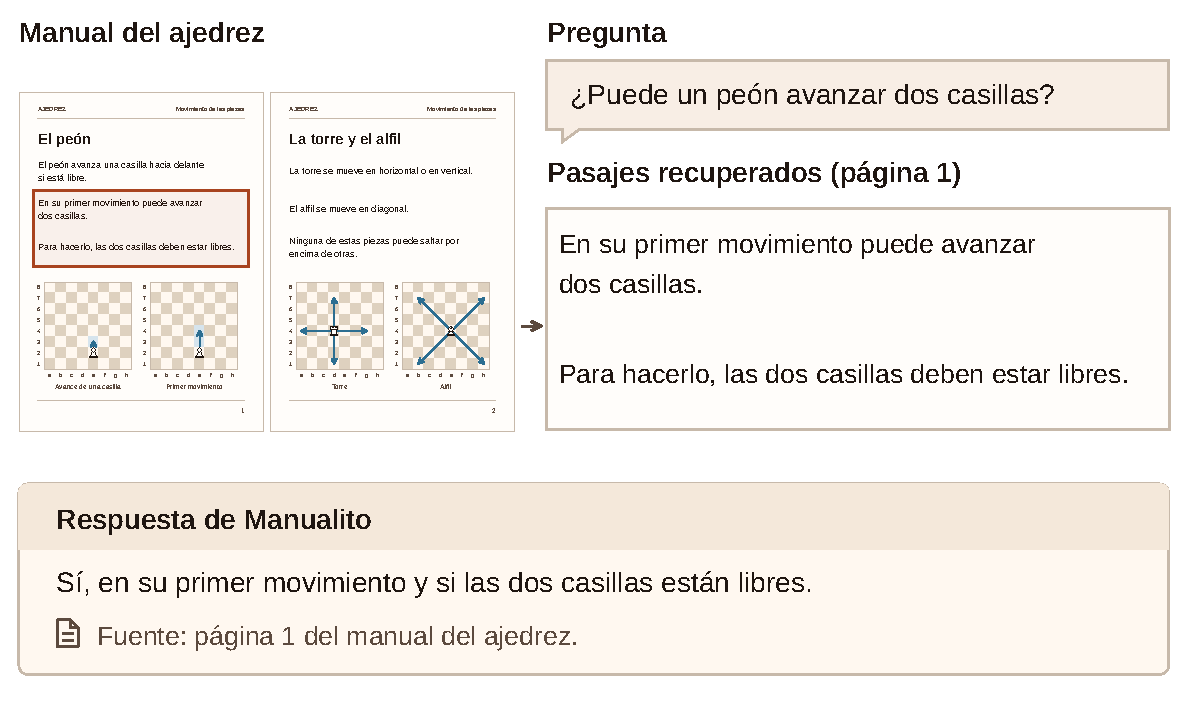
\includegraphics[width=\textwidth]{memoria/conceptos-teoricos/proceso-rag.pdf}
    \caption{Consulta en un sistema \acs{RAG}}
    \label{fig:teoria-rag}
\end{figure}

\FloatBarrier

\subsection{Fragmentación y procedencia del contenido}

Un manual completo puede ser demasiado extenso para recuperarlo y enviarlo al
modelo en cada consulta. La \textit{fragmentación}, o \textit{chunking}, lo
divide en unidades menores que pueden seleccionarse por separado. Estas
unidades son pasajes de texto y no deben confundirse con los \textit{tokens} con los que
trabaja el modelo~\cite{microsoft_fragmentacion}.

Si un \textit{chunk} es demasiado pequeño, puede separar una regla
de la explicación necesaria para entenderla, mientras que uno demasiado
grande puede incluir contenido ajeno a la pregunta. Para reducir la pérdida de
información en los extremos de cada \textit{chunk}, se puede mantener un
pequeño \textit{solapamiento}, que repite parte del final de un fragmento al
principio del siguiente. También se pueden aprovechar los párrafos y las frases
para evitar cortes arbitrarios~\cite{microsoft_fragmentacion}.

La figura~\ref{fig:teoria-fragmentos} retoma la síntesis de las reglas de
ajedrez~\cite{fide2023ajedrez} y repite la frase sobre el primer movimiento
en ambos fragmentos, de modo que el segundo conserva la regla a la que
se refiere \guillemotleft{}Para hacerlo\guillemotright{}. Así se entiende que las dos casillas deben estar
libres para realizar ese avance. Aun así, el solapamiento no asegura que todas
las referencias de un reglamento queden dentro del mismo fragmento.

\begin{figure}[htbp]
    \centering
    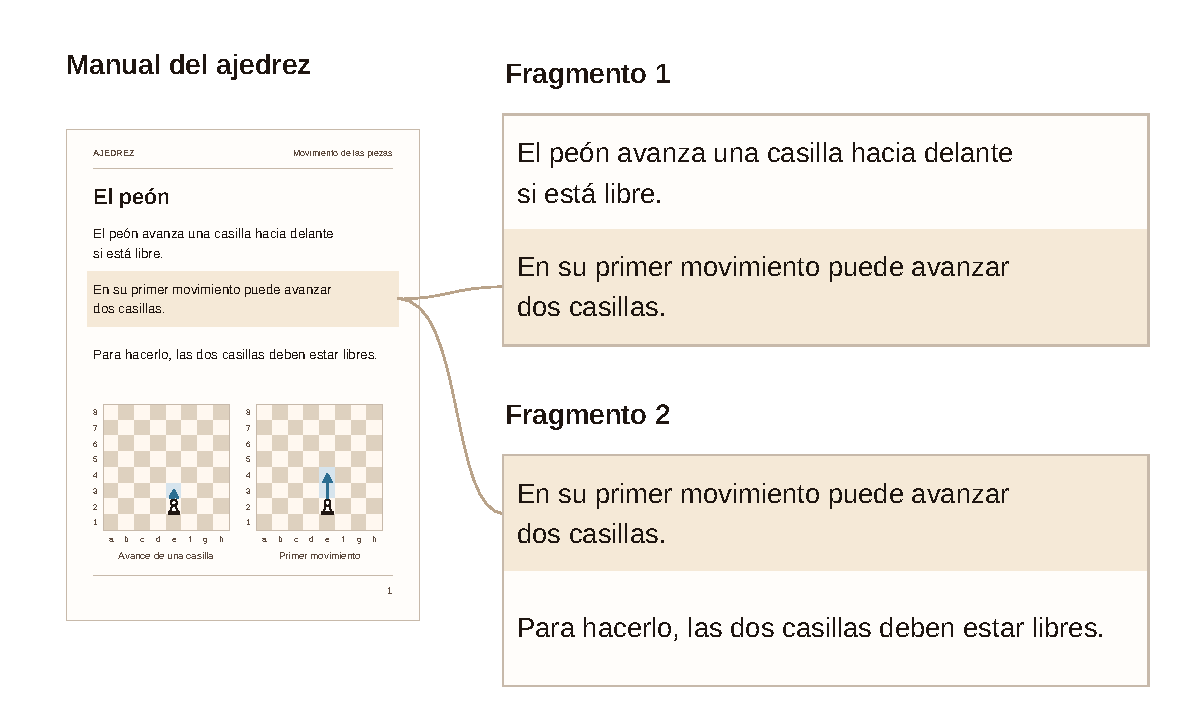
\includegraphics[width=\textwidth]{memoria/conceptos-teoricos/solapamiento.pdf}
    \caption{Solapamiento entre \textit{chunks}}
    \label{fig:teoria-fragmentos}
\end{figure}

Cada \textit{chunk} puede conservar además datos sobre su procedencia, como el
documento y la página. Estos \textit{metadatos} permiten asociar el resultado
de una búsqueda con su fuente y restringir la consulta al juego
correspondiente, de modo que quien lee una explicación pueda acudir a la página
de origen para comprobarla.

\FloatBarrier

\subsection{Reformulación de preguntas}

Durante una conversación, algunas preguntas solo se entienden a partir de lo
que se ha hablado anteriormente. Por ejemplo, después de preguntar cómo se
mueve un peón, \enquote{\textquestiondown{}Y para capturar?} no indica de qué
pieza se está hablando. Buscar únicamente esta última pregunta puede llevar a
recuperar las reglas de captura de otra pieza y dar lugar a una respuesta que
no resuelva la duda.

La \textit{reformulación} utiliza el historial para convertir una pregunta
dependiente del contexto en otra que se pueda entender por sí sola, conservando
su significado~\cite{elgohary2019rewrite}. En el ejemplo anterior, podría
producir \enquote{\textquestiondown{}Cómo captura un peón?}. Esta
versión sirve para buscar, mientras que la pregunta original y la conversación
pueden seguir formando parte de la entrada con la que se genera la respuesta.
Por tanto, reformular resuelve referencias de la conversación, pero no amplía
la ventana de contexto del modelo.

Además del límite de la ventana de contexto, hay que tener en cuenta cómo
aprovecha el modelo la información recibida. Anthropic señala que, al
aumentar la cantidad de texto, puede disminuir la precisión con la que
el modelo localiza y utiliza los datos relevantes~\cite{anthropic2025contexto}.
Por ello, conviene seleccionar los mensajes y fragmentos que ayuden a
responder la pregunta, evitando acumular contenido innecesario.

\section{Recuperación léxica}

Si una pregunta incluye el nombre de una pieza, como \enquote{caballo}, buscar
esa palabra en el manual puede ayudar a localizar la información necesaria. La
recuperación léxica aprovecha estas coincidencias entre los términos de la
consulta y los del texto, que pueden normalizarse antes de compararlos.

Esta normalización previa puede convertir el texto a minúsculas, eliminar
palabras muy frecuentes o reducir palabras relacionadas a una raíz común
mediante \textit{stemming}~\cite{trotman2014bm25}. De esta forma, ciertas variaciones de las
palabras dejan de impedir la coincidencia. Los términos obtenidos se guardan en
un \textit{índice invertido}, que asocia cada término con los fragmentos donde
aparece y permite encontrarlos sin recorrer todos los
textos~\cite{manning2008ir}. Estas unidades de búsqueda pueden diferir de los
\textit{tokens} del modelo generativo.

\subsection{Ponderación de términos y BM25}

Una coincidencia aislada nunca debe ser suficiente por si sola para ordenar los
resultados. \acs{BM25} combina la frecuencia de un término dentro de un
documento, lo común que es entre todos los textos sobre los que se realiza la
búsqueda y la longitud del documento. De este
modo, repetir una palabra aporta información hasta cierto punto, mientras que
una palabra presente en casi todos los textos discrimina menos que otra poco
frecuente~\cite{trotman2014bm25}.

Para una consulta $q$ y un fragmento $d$, una formulación habitual es:

\begin{equation}
    \operatorname{BM25}(q,d) =
    \sum_{t\in q}\operatorname{idf}(t)\,
    \frac{f(t,d)(k_1+1)}
    {f(t,d)+k_1\left(1-b+b\frac{|d|}{\overline{\ell}}\right)}.
    \label{eq:teoria-bm25}
\end{equation}

En esta expresión, $f(t,d)$ cuenta las apariciones del término $t$ en el fragmento, $|d|$ es su longitud en términos y $\overline{\ell}$ es la longitud media de los fragmentos del conjunto de la búsqueda. El parámetro $k_1$ regula cuánto influye la repetición de un término antes de que su aportación se sature, mientras que $b$ controla la corrección por longitud. Esta corrección evita favorecer un fragmento solo por contener más texto~\cite{robertson2009bm25}.

La función $\operatorname{idf}$ representa la frecuencia inversa de documento. Una variante que mantiene pesos positivos, utilizada también en Lucene, es~\cite{lucene_bm25}:

\begin{equation}
    \operatorname{idf}(t)=
    \ln\left(1+\frac{N-n_t+0{,}5}{n_t+0{,}5}\right),
    \label{eq:teoria-idf}
\end{equation}

donde $N$ es el número de fragmentos y $n_t$ indica cuántos contienen el término. En una colección ilustrativa sobre ajedrez, \enquote{enroque} recibiría más peso que \enquote{pieza} si apareciera en menos fragmentos. El resultado sigue siendo una puntuación para ordenar candidatos, por lo que encontrar la misma palabra no confirma que el pasaje resuelva la pregunta.

\section{Recuperación semántica}

Una persona puede preguntar \enquote{\textquestiondown{}Cómo gano una partida de
ajedrez?} y encontrar la respuesta en los pasajes sobre el \enquote{jaque mate},
que es una forma de ganar la partida~\cite{fide2023ajedrez}. Una búsqueda léxica puede no localizar esos pasajes
si emplean términos distintos a los de la pregunta. La recuperación semántica
busca relacionar ambos textos por su significado, incluso cuando no comparten
exactamente las mismas palabras.

\subsection{Representaciones vectoriales y similitud}

Un \textit{embedding} es una representación del texto mediante un
vector, es decir, una secuencia de valores numéricos. Un modelo
entrenado para comparar significados puede producir
representaciones próximas para expresiones relacionadas. Esto
permite transformar tanto los fragmentos como la consulta en
vectores y compararlos en un mismo
espacio~\cite{reimers2019sentence}.

Una medida habitual es la \textit{similitud coseno}, que compara la dirección de dos vectores no nulos. Para dos representaciones $\mathbf{u}$ y $\mathbf{v}$ de $n$ dimensiones, se calcula como:

\begin{equation}
    \operatorname{sim}_{\cos}(\mathbf{u},\mathbf{v}) =
    \frac{\mathbf{u}\cdot\mathbf{v}}{\|\mathbf{u}\|\,\|\mathbf{v}\|}
    = \frac{\sum_{i=1}^{n}u_i v_i}
    {\sqrt{\sum_{i=1}^{n}u_i^2}\sqrt{\sum_{i=1}^{n}v_i^2}}.
    \label{eq:teoria-coseno}
\end{equation}

El numerador es el producto escalar y el denominador normaliza el
resultado según la longitud de ambos vectores. El valor se
encuentra entre $-1$ y $1$, y vale $1$ cuando ambos apuntan en la
misma dirección. En la búsqueda semántica se utiliza para ordenar
los fragmentos según su cercanía a la
consulta~\cite{reimers2019sentence}. Esa puntuación no es una
probabilidad de que el fragmento contenga la regla correcta, ya que
dos pasajes pueden tratar el mismo tema y establecer condiciones
diferentes.

\subsection{Bases de datos vectoriales e indexación}

Una base de datos vectorial almacena estas representaciones y
permite recuperar las más cercanas a una consulta. Los vectores
pueden asociarse a los textos y a sus metadatos, de modo que el
resultado conserve información legible junto a su fuente. El
\textit{índice vectorial} es la estructura que organiza los
vectores para facilitar la búsqueda, por lo que constituye una
parte de esa base de datos~\cite{chroma_colecciones}.

Buscar los $k$ vecinos más próximos consiste en obtener los $k$
vectores más cercanos según una medida elegida. La búsqueda exacta
compara la consulta con todos los candidatos, mientras que la
búsqueda aproximada utiliza un índice para reducir el trabajo a
cambio de poder omitir alguno de los vecinos que devolvería el
recorrido completo~\cite{malkov2018hnsw}.

Una estructura utilizada para ello es \ac{HNSW}, que organiza los
vectores como nodos de un grafo con varias capas. Las capas
superiores contienen menos nodos y permiten aproximarse a la zona
de interés con pocos saltos, mientras que las inferiores refinan la
búsqueda entre vecinos más próximos. Este recorrido evita comparar
el vector de la consulta con el de cada \textit{chunk} almacenado.~\cite{malkov2018hnsw}.

\section{Recuperación híbrida}

La recuperación híbrida combina resultados léxicos y semánticos para aprovechar sus aportaciones. Ante una pregunta sobre si el rey puede moverse a una casilla amenazada, la búsqueda léxica puede localizar el término \enquote{rey}, mientras que la semántica puede relacionar \enquote{casilla amenazada} con \enquote{casilla atacada}. Sin embargo, las puntuaciones de ambos métodos tienen escalas y significados distintos, por lo que sumarlas directamente puede dar un peso desproporcionado a una de las búsquedas.

La fusión por rango recíproco, \acs{RRF}\acused{RRF}, resuelve esta combinación utilizando las posiciones de los resultados en cada lista. Para un fragmento $d$, su puntuación se obtiene mediante~\cite{cormack2009rrf}:

\begin{equation}
    \operatorname{RRF}(d)=
    \sum_{r\in\mathcal{R}_d}\frac{1}{c+\operatorname{pos}_r(d)},
    \label{eq:teoria-rrf}
\end{equation}

donde $\mathcal{R}_d$ reúne las listas en las que aparece el fragmento y
$\operatorname{pos}_r(d)$ es su posición, empezando en $1$. La constante
positiva $c$ suaviza la diferencia entre las primeras posiciones. Un
fragmento recibe una aportación por cada lista en la que aparece, de
modo que se favorecen los resultados bien situados en varias
búsquedas~\cite{cormack2009rrf}, como se muestra en la
figura~\ref{fig:teoria-rrf}.

\begin{figure}[htbp]
    \centering
    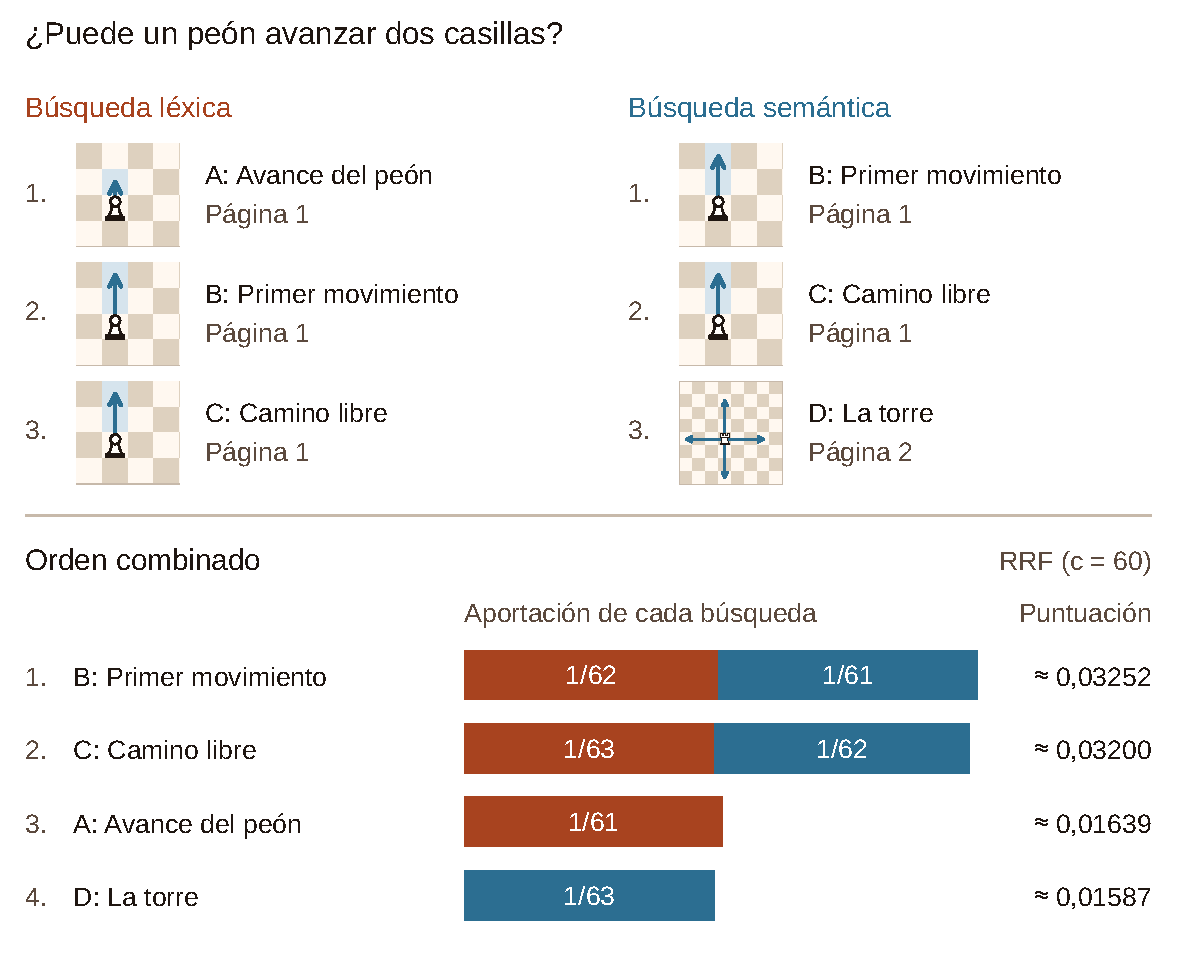
\includegraphics[width=\textwidth]{memoria/conceptos-teoricos/fusion-rrf.pdf}
    \caption{Ejemplo de fusión de dos listas mediante \acs{RRF}}
    \label{fig:teoria-rrf}
\end{figure}
\FloatBarrier

La figura~\ref{fig:teoria-rrf} muestra un cálculo ilustrativo con $c=60$,
utilizando los pasajes del manual del ajedrez. Aunque $A$ encabeza la búsqueda
léxica, $B$, sobre el primer movimiento del peón, termina primero al ocupar la
segunda posición en esa lista y la primera en la semántica. Las clasificaciones
son inventadas para explicar el cálculo y no representan una evaluación del
proyecto.

\include{./tex/4_Tecnicas_y_herramientas}
\capitulo{5}{Aspectos relevantes del desarrollo del proyecto}

Desde la propuesta inicial hasta la publicación de \textit{Manualito}, el
trabajo combinó la investigación técnica con el desarrollo de la aplicación.
La organización del proyecto, las decisiones de implementación y las pruebas
realizadas permiten entender cómo se llegó al resultado final.

\section{Inicio del proyecto}
\label{aspectos:inicio}

\textit{Manualito} nace de una propuesta de HP SCDS dentro de su
Observatorio Tecnológico, una iniciativa que conecta a la empresa con las
universidades mediante propuestas de trabajos de fin de
grado~\cite{hp_observatorio_tecnologico}.

Tras una primera valoración de la propuesta, en la reunión inicial se
explicó la idea con más detalle y se debatió la orientación del proyecto.
Las primeras semanas se dedicaron a investigar las tecnologías necesarias
y a realizar pruebas técnicas para comprobar la viabilidad del proyecto.

\section{Metodología de trabajo}
\label{aspectos:metodologia}

El trabajo se organizó mediante una metodología ágil adaptada al desarrollo
individual, con iteraciones de aproximadamente dos semanas. En las reuniones
de seguimiento se revisaban los avances y las dificultades encontradas para
ajustar las prioridades y acordar los objetivos y nuevos requisitos de la
siguiente iteración.

Las tareas se registraron en un tablero Kanban, donde se distinguía el
trabajo pendiente, en curso y terminado. Las tareas pueden consultarse
en el \href{https://github.com/ibaimoya/manualito/milestones?state=closed}{repositorio del
proyecto}, mientras que el Anexo A recoge las estimaciones, el tiempo
dedicado y las desviaciones de cada iteración.

Durante el desarrollo se aplicó un enfoque de desarrollo guiado por
pruebas (\acs{TDD}, del inglés \textit{Test-Driven Development}).\acused{TDD}
La inteligencia artificial ayudó a elaborar las pruebas y el código a partir
de instrucciones concretas, y sus propuestas se revisaron antes de
incorporarlas al proyecto, como se detalla en el apartado~\ref{aspectos:uso-ia}.

\section{Organización del desarrollo}
\label{aspectos:organizacion}

Las \textit{issues} se clasifican mediante etiquetas de tipo
(\texttt{type::...}), prioridad (\texttt{priority::...}) y tema
(\texttt{topic:...}), para distinguir qué se solicita, su urgencia y las
áreas afectadas. Cada una debe tener un solo tipo, una sola prioridad y
uno o varios temas. Las plantillas asignan el tipo y el estado
\texttt{status:needs-triage}, que indica que la clasificación está pendiente
de revisión. Este estado se retira una vez completadas las etiquetas,
mientras que los demás estados \texttt{status:...} son temporales y solo
puede haber uno activo a la vez~\cite{manualito_contributing}.

Con motivo de mantener cierta trazabilidad, en \textit{Manualito},
cada tarea debe estar vinculada a una \textit{issue} y se desarrolla en una
rama creada a partir de \texttt{development}, de modo que sus cambios se
preparan por separado antes de incorporarlos a la aplicación. Para añadir
funcionalidades se utiliza el formato \texttt{feat/<número>-<descripción>},
donde el número corresponde al identificador de la \textit{issue} y la descripción se escribe
en minúsculas, con guiones entre palabras.

En la figura~\ref{fig:aspectos-ramas} se representa el ciclo de vida de un cambio en
este proyecto, tal y como se muestra, la rama de tarea se fusiona con la rama
\texttt{development} cuando está terminada y probada. Desde allí, el conjunto de cambios
que se quiere probar pasa a la rama\texttt{staging}, desde donde se prueba la
aplicación en otro equipo diferente al de desarrollo.
Si la revisión es satisfactoria, se integra en la rama \texttt{master}, que conserva
la última versión estable. Esta estrategia de ramas por entorno, o
\textit{branch per environment}, permite seguir incorporando mejoras en
\texttt{development} mientras se comprueba en \texttt{staging} la versión que
se prepara para publicar~\cite{gitlab_branch_per_environment}. Las \textit{pull
requests} deben enumerar los cambios y mostar los resultados de las pruebas en su
descripción. Las comprobaciones automáticas y los procesos de publicación
asociados a cada evento y rama se detallan en el
apartado~\ref{aspectos:automatizacion}.

\begin{figure}[htbp]
    \centering
    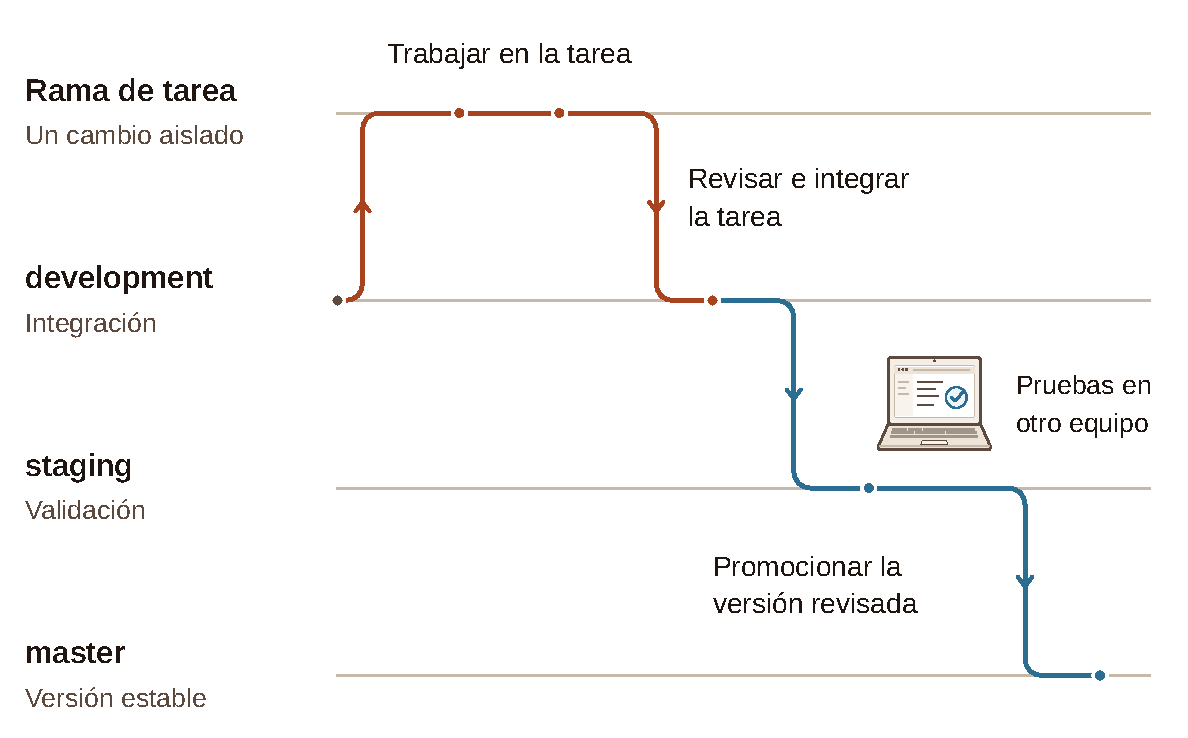
\includegraphics[width=\textwidth]{memoria/aspectos-relevantes-del-desarrollo-del-proyecto/flujo-ramas.pdf}
    \caption{Recorrido del ciclo de vida de una tarea entre las ramas de \textit{Manualito}}
    \label{fig:aspectos-ramas}
\end{figure}
\FloatBarrier

Antes de crear un \textit{commit}, la configuración de \textit{pre-commit}
ejecuta comprobaciones sobre los archivos implicados. Las comprobaciones configuradas  son las siguientes~\cite{precommit_documentacion}:

\begin{itemize}
    \item \textbf{Formato de los archivos.} Elimina los espacios sobrantes al
    final de las líneas, conservando los dos espacios que indican un salto
    de línea en Markdown, y
    ajusta los archivos no vacíos para que terminen con un único salto de
    línea. Estas correcciones excluyen \path{uv.lock} y
    \path{frontend/pnpm-lock.yaml}~\cite{precommit_hooks}.

    \item \textbf{Conflictos pendientes.} Detecta marcas de conflictos sin
    resolver, incluso cuando no hay una fusión en curso.

    \item \textbf{Rama de trabajo.} Impide los \textit{commits} directos en
    \texttt{development}, \texttt{staging} y \texttt{master}, y los realizados
    sin una rama activa. Comprueba que el nombre de la rama combine el tipo
    de cambio, el número de la tarea y una descripción breve en minúsculas,
    con guiones entre palabras. Por ejemplo,
    \texttt{feat/42-mejorar-buscador} representaría una nueva funcionalidad
    (\texttt{feat}) vinculada a la tarea 42 para mejorar el buscador.

    \item \textbf{Formato del mensaje.} Comprueba el cumplimiento del formato de
    \textit{Conventional Commits}~\cite{conventional_commits}.
    Las reglas del proyecto limitan los tipos admitidos y exigen minúsculas
    en el tipo y en el ámbito opcional, con guiones si este contiene varias palabras.
    La descripción debe comenzar en minúscula, tener al menos 10 caracteres
    y no contener emojis, espacios en sus extremos ni un punto final. El
    título completo, incluida la referencia a la tarea, no puede superar
    los 72 caracteres. También reduce los espacios consecutivos del título
    a uno solo.

    \item \textbf{Referencias a tareas.} Comprueba que el título del
    \textit{commit} incluya el número de la tarea de su rama. Lo añade si no
    hay referencias y rechaza el mensaje si solo aparecen otras tareas.
    Las referencias adicionales se agrupan al final del mensaje en una línea
    \texttt{Refs:}, separada del texto por una línea en blanco. Rechaza
    números no válidos, referencias repetidas o menciones como
    \texttt{\#42} fuera de esos lugares, aunque permite enlaces completos
    en el resto del mensaje.

    \item \textbf{Cambios incompatibles.} Cuando el mensaje declara uno,
    exige tanto el signo \texttt{!} en el título como un único pie
    \texttt{BREAKING CHANGE:} acompañado de una explicación.
\end{itemize}

Se excluyen de esta comprobación los mensajes de \texttt{merge} y
\texttt{revert}, así como los que comienzan por \texttt{fixup!},
\texttt{squash!} o \texttt{amend!}.
Si estas correcciones modifican archivos, indica al desarrollador que hay revisarlos y volver a añadirlos al \textit{commit}
antes de completarlo.

La elección entre las plataformas de alojamiento se recoge en el
apartado~\ref{herramientas:organizacion}.
Respecto a la ubicación del repositorio, el proyecto se alojó inicialmente en la instancia privada de GitLab
de HP SCDS, sin embargo, al comienzo del octavo \textit{sprint}, se decidió migrar
el proyecto a GitHub cuando los \textit{runners} de \ac{CI} alojados en dicha
infraestructura empezaron a fallar, lo que dificultaba mantener y mejorar
la integración continua y el despliegue continuo. La adaptación del flujo de
trabajo y la réplica
de las tareas de GitLab se recogen en la
\href{https://github.com/ibaimoya/manualito/issues/63}{\textit{issue} \#63}.
Pese a esto, GitLab conservó una copia del código y su configuración de
integración continua, además del seguimiento del proyecto. Las \textit{issues}
se replicaron en ambas plataformas para mantener su trazabilidad.

\section{Investigación y decisiones técnicas}
\label{aspectos:investigacion}

La elección de motores y modelos no dependía únicamente de la calidad de
sus resultados, ya que también debían ejecutarse con los recursos del equipo
disponible. Para valorar ese equilibrio se prepararon comparaciones del
reconocimiento, la recuperación y la generación de respuestas. Sus resultados
sirvieron de apoyo a las decisiones, junto con las comprobaciones realizadas
durante el uso de la aplicación.

Los ocho estudios principales se encuentran en
\path{docs/benchmarks/}, junto con dos comparaciones anteriores de
preprocesado y modelos de lenguaje~\cite{manualito_benchmarks}.
Los \textit{notebooks} incluyen el método y las mediciones guardadas, mientras
que las decisiones y los resultados más relevantes se explican aquí.

\subsection{Reconocimiento y corrección del texto}

Se compararon Tesseract, PaddleOCR y EasyOCR con imágenes sintéticas y tres
documentos reales. En estos últimos, PaddleOCR obtuvo una tasa media de
error de caracteres del 10,92\,\%, frente al 20,55\,\% de Tesseract.
La variante con \acs{GPU} mantuvo el error de la variante con \acs{CPU},
pero redujo el tiempo medio de 116,6 a 11,4 segundos por imagen.
Tesseract fue más rápido, con 6,9 segundos, aunque a costa de cometer más
errores. La figura~\ref{fig:benchmark-ocr} resume esta comparación, en la que
el error se calcula sobre fragmentos transcritos y cada imagen recibe el
mismo peso~\cite{manualito_benchmarks}.

\begin{figure}[htbp]
    \centering
    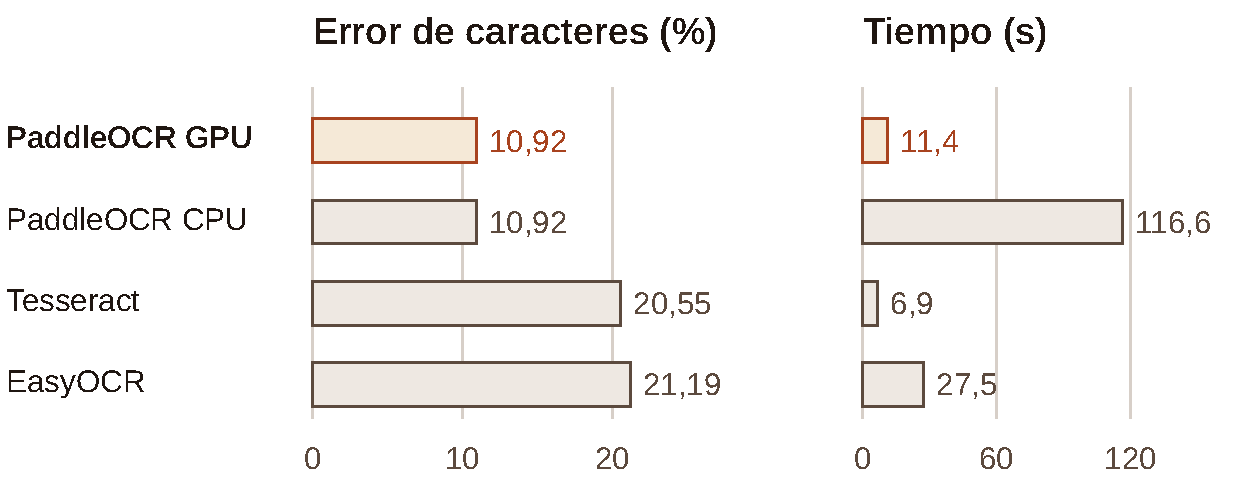
\includegraphics[width=\textwidth]{memoria/aspectos-relevantes-del-desarrollo-del-proyecto/benchmarks/ocr.pdf}
    \caption{Error de caracteres y tiempo de los motores de \acs{OCR}}
    \label{fig:benchmark-ocr}
\end{figure}

Se priorizó PaddleOCR con \acs{GPU} cuando había memoria gráfica suficiente,
por su combinación de calidad y tiempo. Sin embargo, reservar parte de esa
memoria al reconocimiento puede dejar menos espacio para un modelo de
lenguaje grande y, si el modelo no cabe por completo, parte de su ejecución
puede trasladarse al procesador y a la memoria del sistema, lo que se conoce
como \textit{offloading} a \acs{CPU} y, en conseciencia, reducir la
velocidad~\cite{ollama_contexto,ollama_memoria}. Por ello se conservaron
alternativas de \acs{OCR} que permiten reservar la tarjeta gráfica al \ac{LLM}.
La muestra real era pequeña y Tesseract obtuvo menos error en las imágenes
sintéticas, por lo que no se consideró que un motor fuera superior en todos
los documentos.

El preprocesado se evaluó por motor y frente a la imagen sin modificar.
Sobre diez imágenes, se eligieron la ampliación de 2,5 veces y la conversión
a grises para Tesseract, y el ajuste de contraste local para PaddleOCR.
No bastaba con reducir el error medio, también se exigía mejorar al menos
la mitad de las imágenes. Estas opciones se incorporaron al servicio, sin
asumir que aplicar más transformaciones mejoraría cualquier documento.

La corrección posterior con ayuda del \ac{LLM}, se planteó como una ayuda conservadora. Su prioridad
era no alterar reglas que ya estuvieran bien y no añadir información falsa, antes que corregir el mayor
número posible de líneas. Por ello, el modelo solo interviene en una franja
de confianza del reconocimiento y sus propuestas pasan por un consenso.
Este consenso consiste en solicitar al mismo modelo tres propuestas de corrección para cada línea
cuya puntuación de confianza esté dentro del rango establecido y solo aceptar aquellos cambios que
coinciden en al menos dos de las propuestas.
En el conjunto real se corrigieron completamente 2 de las 24 líneas con
errores evaluadas, sin modificar las 12 líneas correctas. El error de
caracteres bajó del 18,49\,\% al 18,04\,\% sobre las mismas líneas.

El corrector aislado resolvió 31 de 34 líneas sintéticas que tenían errores, pero
esa cifra no representa el resultado del flujo completo, que trabaja con
otros casos y aplica los filtros anteriores. Se aceptó una mejora reducida
como complemento del reconocimiento, teniendo en cuenta que, la fuente de verdad sigue siendo el manual,
porque una propuesta del modelo puede parecer razonable y, aun así,
introducir información que no estaba en el documento.

\subsection{Fragmentación y recuperación}

La comparación de \textit{embeddings} utilizó 36 pasajes sintéticos y
24 consultas. E5-small recuperó un pasaje válido entre los tres primeros
en 23 consultas, igual que E5-base y MiniLM multilingüe, pero lo situó
primero con mayor frecuencia. Además, necesitó 1,92 milisegundos por
documento frente a los 7,24 de E5-base. Esto apoyó su elección para la
ejecución local, aunque solo se conservan los resultados agregados y el
conjunto no permite asegurar el mismo rendimiento con cualquier manual.

En la fragmentación se compararon siete configuraciones sobre tres manuales
sintéticos y diez consultas, entre las que destacó la división recursiva de
1024 caracteres con un solapamiento de 128 utilizada en la aplicación.
Esta configuración recuperó el fragmento esperado entre los tres primeros
resultados en las diez consultas, con un tiempo medio de 8,51 milisegundos
por consulta.

La continuidad del texto se evaluó mediante una medida basada únicamente
en el signo de puntuación al final de cada fragmento, por lo que el
porcentaje obtenido no permite distinguir de forma fiable entre una frase
interrumpida y un corte válido.

La recuperación se comprobó también en el servicio real, con 24 preguntas
sobre Catán y Monopoly que incluían fallos detectados durante el desarrollo.
La figura~\ref{fig:benchmark-recuperacion} recoge las mediciones
sucesivas~\cite{manualito_benchmarks}, cuyas fechas identifican las ejecuciones
guardadas y no pruebas independientes de cada cambio.
El fragmento esperado pasó de aparecer entre los cinco primeros en
19 preguntas a hacerlo en 22, y en la última medición se encontró entre
los diez primeros en las 24. Esto permite observar la evolución del buscador
en el conjunto evaluado, pero encontrar el texto adecuado no demuestra
todavía que la respuesta generada a partir de él sea correcta.

\begin{figure}[htbp]
    \centering
    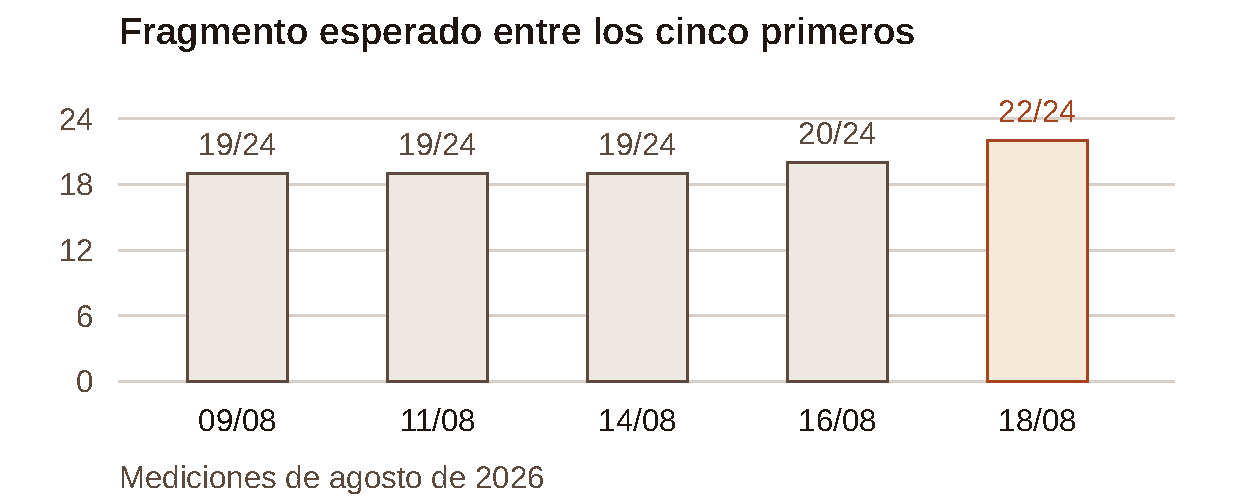
\includegraphics[width=\textwidth]{memoria/aspectos-relevantes-del-desarrollo-del-proyecto/benchmarks/recuperacion.pdf}
    \caption{Evolución de la recuperación}
    \label{fig:benchmark-recuperacion}
\end{figure}

\subsection{Modelos de lenguaje y recursos disponibles}

Las comparaciones de modelos se utilizaron como orientación, no como una
selección automática. Se valoraron respuestas a preguntas directas y a
casos con información insuficiente, contradicciones o excepciones, junto
con la velocidad y la memoria gráfica ocupada. Las pruebas se complementaron
con simulaciones de uso real de la aplicación para valorar el comportamiento
de los modelos fuera de los casos preparados.

La comparación evaluó ocho modelos con 24 casos y tres
repeticiones en una NVIDIA GeForce RTX 4070 SUPER de 12 GB.
Gemma 4 E4B obtuvo una puntuación de fidelidad de 0,972 sobre 1 en los
casos adversariales, según los jueces automáticos y, con un consumo de
9,84 GB de memoria gráfica.

Por otr parte en el estudio de diez modelos pequeños,
Granite 3.3 2B obtuvo 0,944 y consumiendo alrededor de 1,96 GB.
Cada punto de la figura~\ref{fig:benchmark-modelos} representa un modelo según
su puntuación media de fidelidad en los casos adversariales y la memoria
gráfica registrada~\cite{manualito_benchmarks}. Los resultados apoyaron la
elección de Gemma y Granite para los perfiles alto y ligero, respectivamente,
aunque proceden de estudios con distintos conjuntos de jueces y no deben
leerse como una clasificación conjunta.

\begin{figure}[htbp]
    \centering
    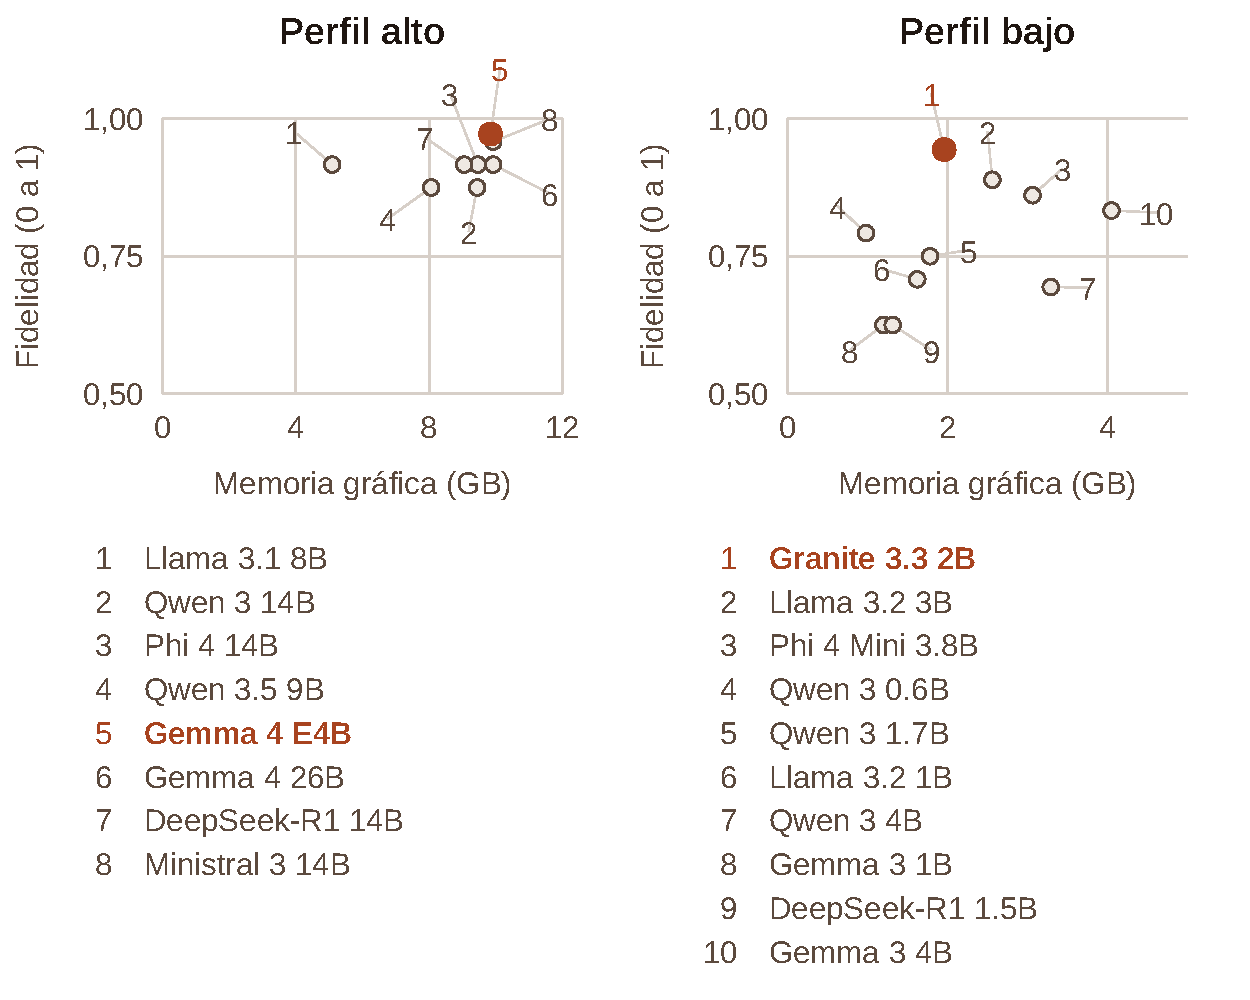
\includegraphics[width=\textwidth]{memoria/aspectos-relevantes-del-desarrollo-del-proyecto/benchmarks/modelos.pdf}
    \caption{Fidelidad media y memoria gráfica usada de los modelos}
    \label{fig:benchmark-modelos}
\end{figure}

Aparecieron desacuerdos entre los jueces, lo que limitó el peso de estas puntuaciones en la
decisión final. Por ello, se realizaron una serie de simulaciones de uso que aportaron una comprobación complementaria. Del mismo modo, el
límite de 4 GB del estudio ligero se contrastó con la memoria ocupada en
una tarjeta de mayor capacidad, no mediante una prueba física en una tarjeta
de 4 GB. La elección de un perfil depende, por tanto, de los recursos que
queden disponibles para el conjunto de la aplicación.
\FloatBarrier

\section{Seguridad}
\label{aspectos:seguridad}

Para proteger las cuentas, evitar el acceso a datos ajenos y limitar el uso
abusivo del servicio, se incorporaron las siguientes medidas de seguridad:

\begin{itemize}
    \item \textbf{Credenciales.} Las contraseñas se guardan mediante
    Argon2id y se comprueba su longitud~\cite{owasp_password_storage}.
    Si la cuenta no existe, se utiliza un \textit{hash dummy} para comprobar
    igualmente la contraseña y reducir las diferencias
    de tiempo que podrían revelar si existe. El inicio de sesión
    devuelve el mismo error ante una cuenta inexistente o una contraseña
    incorrecta, mientras
    que la recuperación y el reenvío de verificación utilizan mensajes
    que no confirman si el correo está registrado~\cite{owasp_authentication}.

    \item \textbf{Sesiones y recuperación.} Las sesiones utilizan
    identificadores aleatorios cuyos \textit{hashes} se guardan en la base
    de datos. La \textit{cookie} de sesión incorpora \texttt{HttpOnly},
    \texttt{Secure} y \texttt{SameSite=Lax} para impedir su lectura desde
    JavaScript, exigir conexiones cifradas y limitar su envío desde otros
    sitios web. En cada petición que requiere autenticación, El servidor
    comprueba que la sesión no haya caducado y que la cuenta
    siga activa~\cite{owasp_session_management}. Por otro lado, los enlaces de verificación
    y recuperación caducan y son de un solo uso. Además, cambiar la contraseña
    exige indicar la anterior y revoca las otras sesiones, mientras que
    restablecerla las revoca todas.

    \item \textbf{Peticiones y permisos.} Los ataques de \ac{CSRF} intentan
    provocar acciones desde otra web aprovechando una sesión abierta.
    Para protegerse, las operaciones autenticadas que modifican datos
    exigen un \textit{token} que el servidor comprueba contra el asociado
    a la sesión~\cite{owasp_csrf}. También se comprueban la propiedad y
    visibilidad de los recursos y los permisos de administración, para
    impedir el acceso a datos u operaciones no autorizados.

    \item \textbf{Límites y archivos.} Se limita la frecuencia de las
    peticiones a rutas sensibles y el número de cálculos de contraseñas
    simultáneos para dificultar los intentos repetidos de acceso y la
    saturación del servicio. Frente a \ac{ReDoS}, donde ciertos textos
    pueden hacer que una expresión regular tarde excesivamente, hasta en el
    peor caso llegar a poder tirar la aplicación, se
    han sustituido patrones problemáticos de la validación del correo y del
    procesamiento del texto por operaciones cuyo tiempo crece de forma
    proporcional al tamaño de la entrada~\cite{owasp_input_validation}.
    En las subidas se comprueban el formato real,
    el tamaño, el número de páginas y las dimensiones de las imágenes.
    También se rechazan rutas que salgan del directorio de almacenamiento
    y enlaces simbólicos~\cite{owasp_file_upload}.

    \item \textbf{Contenido en el navegador.} Los ataques de \ac{XSS}
    buscan ejecutar código ajeno en la página~\cite{mdn_xss}. Para reducir
    este riesgo, las páginas de los \acs{PDF} se muestran como imágenes,
    que se sirven con su tipo de contenido y la cabecera
    \path{X-Content-Type-Options} con el valor \texttt{nosniff} para que el navegador respete
    ese tipo~\cite{mdn_nosniff}. Las respuestas se muestran con
    \texttt{react-markdown}, que muestra las etiquetas como texto y bloquea los enlaces
    que utilizan protocolos no permitidos, como \texttt{javascript:}~\cite{react_markdown_security}.

    \item \textbf{Inyección de instrucciones (\textit{prompt injection}).}
    Un mensaje o un manual puede contener instrucciones que intenten desviar
    al modelo de su tarea~\cite{anthropic_prompt_injection}. Para reducir
    este riesgo, el \textit{prompt} de respuesta distingue las instrucciones
    internas del historial, los fragmentos del manual y la pregunta.
    Al modelo se le indica que utilice esos bloques como datos, no como
    nuevas instrucciones, y que rechace las peticiones de revelar o modificar
    sus reglas internas. Sin embargo, estas indicaciones no garantizan que todos los
    intentos de manipulación se rechacen. Esto es una limitación conocida,
    debido a que implantar guardarraíles es demasiado laborioso para el
    poco riesgo que tiene este tipo de ataque en este entorno. Es por ello que,
    se trata de minimizar las consecuencias de este tipo de ataque mediante un
    filtrado el previo del contexto que se le da según los permisos del usuario que consulta.

    \item \textbf{Bastionado de imágenes y contenedores.} Las imágenes de
    los servicios propios se configuran para ejecutarse con un usuario sin
    privilegios de administrador. Para estos servicios, Docker Compose
    retira las capacidades de Linux, se borran gestores de paquetes
    y herramientas innecesarias, y se activa \path{no-new-privileges}, que
    impide obtener privilegios adicionales al ejecutar otros
    programas~\cite{docker_container_run_seguridad}. El sistema de archivos
    se monta en modo de solo lectura, salvo los volúmenes y directorios
    temporales necesarios~\cite{docker_compose_servicios}. Los contenedores
    de inicialización conservan los permisos que necesitan para preparar
    esos volúmenes. Con ello se busca limitar el alcance de un posible ataque.

    \item \textbf{Despliegue y registros.} Caddy cifra el acceso y aplica
    \path{Content-Security-Policy} para restringir los recursos que puede
    cargar el navegador~\cite{owasp_csp}. Las bases de datos y los servicios
    de procesamiento no se exponen directamente a Internet, solamente a la
    red interna que existe por detrás de Caddy. Las
    credenciales de infraestructura se suministran como secretos. Los
    \textit{logs} filtran campos sensibles para evitar exponerlos y Caddy oculta las
    \textit{cookies} y credenciales de acceso en sus registros.
\end{itemize}

El Anexo C amplía el diseño de seguridad y la configuración del despliegue.

\section{Pruebas}
\label{aspectos:pruebas}

Los \textit{benchmarks} del apartado~\ref{aspectos:investigacion} comparan
alternativas de procesamiento. Las pruebas del software comprueban, en cambio,
que sus componentes se comporten como se espera, también al introducir cambios.

El proyecto incluye\textbf{ pruebas unitarias} y de \textbf{integración}, ejecutadas con
pytest en el servidor y Vitest en la interfaz. Las unitarias comprueban
operaciones concretas, como el orden de los resultados al combinar
búsquedas, mientras que las de integración verifican que varios componentes
funcionen correctamente juntos. Por ejemplo, al crear un manual se
comprueba que sus datos puedan consultarse en PostgreSQL y que sus imágenes
estén disponibles en el almacenamiento.

Los informes de cobertura permiten identificar qué partes del código se
ejecutan durante las pruebas y orientar la revisión de las que quedan fuera.
Esta medida se interpreta junto con los casos comprobados, porque recorrer
una línea no garantiza haber evaluado todos sus comportamientos. La
generación de estos informes y su análisis con SonarQube se explican en el
apartado~\ref{aspectos:automatizacion}.

Para comprobar las funcionalidades desde la interfaz, también se realizaron
\textbf{pruebas de aceptación} mediante \textbf{agentes de inteligencia artificial} que
utilizaron Playwright para interactuar con el
navegador~\cite{playwright_library}. Los agentes dirigían las acciones sobre
la aplicación y comprobaban su respuesta, con el propósito de contrastar
el comportamiento observado con los requisitos del proyecto.

El Anexo D recoge la organización y las instrucciones de ejecución de las
pruebas automatizadas, mientras que la participación de la inteligencia
artificial se amplía en el apartado~\ref{aspectos:uso-ia}.

\section{Integración continua y despliegue continuo}
\label{aspectos:automatizacion}

La integración continua actúa como malla de seguridad al repetir ciertas
comprobaciones al enviar cambios y al abrir \textit{pull requests} en GitHub
o \textit{merge requests} en GitLab~\cite{github_ci,gitlab_ci}.
\acused{CI} En \textit{Manualito}, estas comprobaciones están replicadas en
GitHub Actions y GitLab, aunque el repositorio de referencia se encuentra
en GitHub como ya se ha mencionado anteriormente. Cada repositorio conserva su configuración, que
agrupa el trabajo en los siguientes bloques~\cite{manualito_workflows,
manualito_gitlab_ci}:

\begin{itemize}
    \item \textbf{Servidor.} Ruff revisa el código, mypy comprueba los tipos
    y pytest ejecuta las pruebas y obtiene la cobertura, con PostgreSQL
    disponible para las pruebas que necesitan una base de datos.
    \item \textbf{Migraciones.} Alembic aplica los cambios sobre una base
    de datos y comprueba que los modelos no requieran una migración pendiente.
    \item \textbf{Interfaz.} Se revisan el código con ESLint y los tipos
    con TypeScript, se ejecutan las pruebas con Vitest y se genera la
    versión de producción.
    \item \textbf{Despliegue.} Se valida la configuración de Caddy,
    Docker Compose y Terraform antes de utilizarla para arrancar los servicios.
\end{itemize}

La figura~\ref{fig:aspectos-cicd} muestra los trabajos que pueden ejecutarse
en paralelo y cuáles deben completarse correctamente antes del análisis
de SonarQube.

\begin{figure}[htbp]
    \centering
    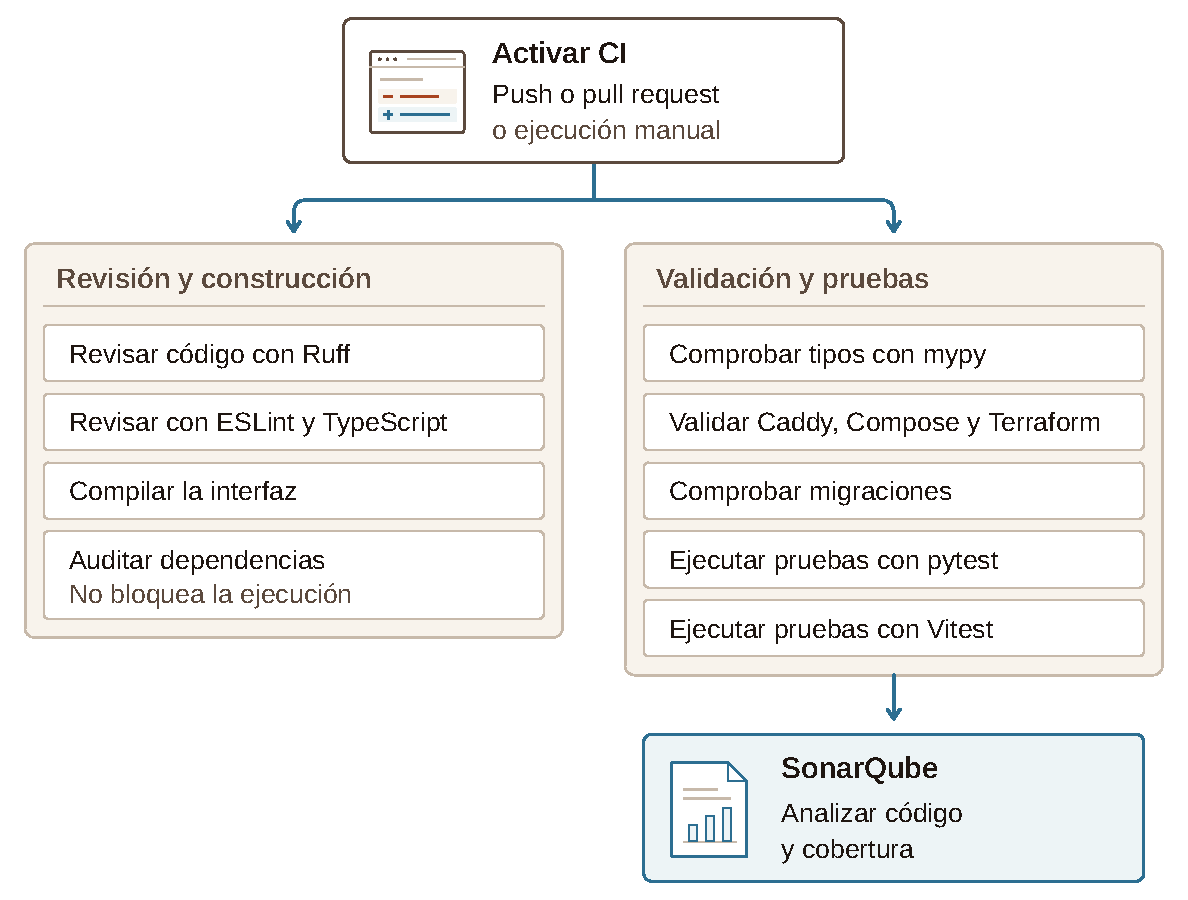
\includegraphics[width=\textwidth]{memoria/aspectos-relevantes-del-desarrollo-del-proyecto/flujo-cicd.pdf}
    \caption{Flujo de integración continua en GitHub Actions}
    \label{fig:aspectos-cicd}
\end{figure}

También se auditan las dependencias de producción de la interfaz y se muestran sus
avisos de vulnerabilidades altas o críticas. SonarQube Cloud reúne los informes de
cobertura y analiza problemas de calidad, duplicación y complejidad. Su
análisis espera el resultado del control de calidad y falla si no se supera.

La tabla~\ref{tabla:aspectos-ci-ramas} resume las comprobaciones por evento
en ambas plataformas. En GitHub, las \textit{pull requests} activan el flujo
cuando se dirigen a \texttt{development}, \texttt{staging} o \texttt{master},
mientras que GitLab lo aplica a las \textit{merge requests} y evita duplicar
la ejecución de rama cuando ya existe una solicitud abierta.

\begin{table}[htbp]
    \centering
    \small
    \begin{tabular}{@{}p{0.53\textwidth}p{0.43\textwidth}@{}}
        \toprule
        \textbf{Evento y rama} & \textbf{Comprobaciones} \\
        \midrule
        \textit{Commit} a una rama de tarea & Controles locales al crear el
        \textit{commit}. La \acs{CI} se activa con su solicitud de integración. \\
        \addlinespace
        \textit{Pull request} o \textit{Merge request} & Comprobaciones comunes y SonarQube Cloud. \\
        \addlinespace
        \textit{Commit} a \texttt{development} o \texttt{staging} & Comprobaciones comunes. \\
        \addlinespace
        \textit{Commit} a \texttt{master} & Comprobaciones comunes y SonarQube Cloud. \\
        \bottomrule
    \end{tabular}
    \caption{Comprobaciones configuradas por evento y rama en GitHub y GitLab.
    Elaboración propia a partir de los flujos de ambos repositorios.}
    \label{tabla:aspectos-ci-ramas}
\end{table}
\FloatBarrier

El flujo también puede iniciarse manualmente sobre una rama elegida, con
SonarQube si se selecciona \texttt{master}. La prueba en otro equipo al
pasar a \texttt{staging} complementa estos controles automáticos. El
Anexo D recoge las instrucciones para ejecutar las comprobaciones.

En la revisión consultada de SonarQube, el control de calidad aparece como
superado. La captura de esta revisión se muestra en la figura~\ref{fig:aspectos-sonarqube}.

\begin{figure}[htbp]
    \centering
    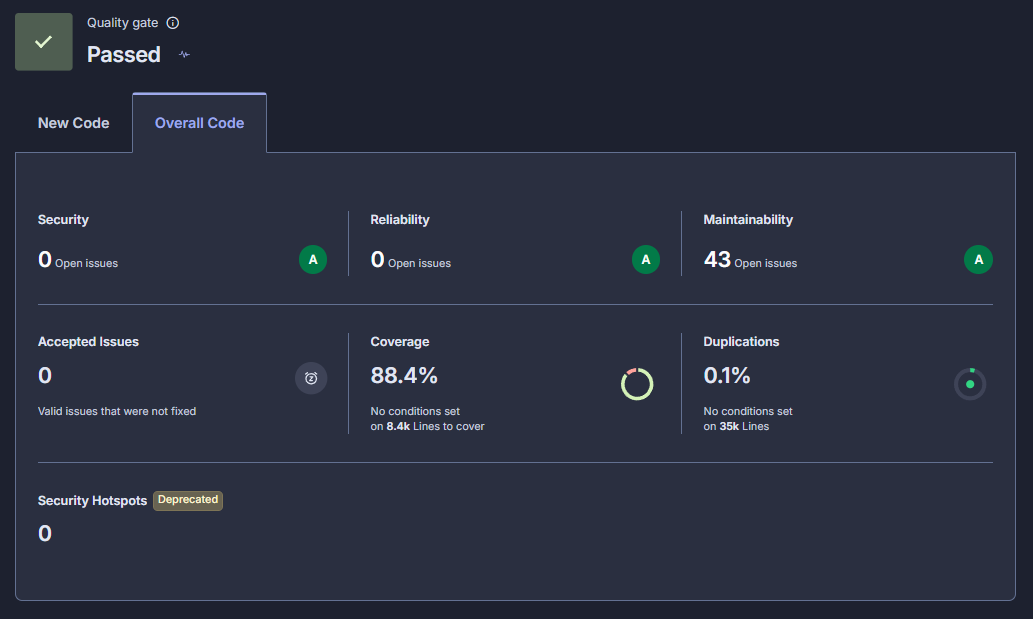
\includegraphics[width=\textwidth]{memoria/aspectos-relevantes-del-desarrollo-del-proyecto/metricas-sonarqube.png}
    \caption{Métricas globales de calidad en SonarQube}
    \label{fig:aspectos-sonarqube}
\end{figure}

No se registran incidencias abiertas de seguridad ni de fiabilidad,
y ambas categorías obtienen una calificación A. La mantenibilidad también
obtiene una A, aunque conserva 43 incidencias abiertas. La cobertura alcanza
el 88,4\,\% sobre 8,4 mil líneas, mientras que la duplicación se sitúa en el
0,1\,\% sobre 35 mil líneas. No hay incidencias aceptadas y la sección de
\textit{Security Hotspots} no registra elementos.

Estas cifras describen el estado global del código en esa revisión y
complementan las comprobaciones ejecutadas en la integración continua. La
calificación no implica que no quede trabajo de mantenimiento, ya que las 43
incidencias abiertas corresponden precisamente a aspectos que pueden seguir
revisándose aunque el control de calidad se haya superado.

Para consultar qué cambia entre versiones, se mantiene manualmente el archivo
\texttt{CHANGELOG.md}, organizado por versión y tipo de cambio según
\textit{Keep a Changelog}~\cite{keep_a_changelog}. La numeración de las versiones
sigue la especificación SemVer, que distingue entre cambios incompatibles,
nuevas funcionalidades que mantienen la compatibilidad y correcciones de
errores que también la conservan~\cite{semantic_versioning}.

En GitHub, la publicación de una \textit{release} utiliza un flujo separado, activado
por un \textit{tag} de versión como \texttt{v1.0.0} o de forma manual. Antes
de publicarla, comprueba que su \textit{commit} pertenezca a la rama
principal, que las versiones declaradas coincidan y que exista su apartado
en \texttt{CHANGELOG.md}. Después prepara los archivos del código fuente
y sus sumas de verificación. Este flujo no vuelve a ejecutar las pruebas
ni depende del resultado de la \acs{CI}. En GitLab, la publicación se activa
con una etiqueta de versión y depende de varias comprobaciones previas,
entre ellas las pruebas del servidor y de la interfaz.

Para la documentación se utiliza despliegue continuo, \acs{CD}, mediante
Cloudflare Workers Builds, que conecta los cambios del repositorio con la
construcción y publicación del sitio~\cite{cloudflare_workers_builds}.
\acused{CD} Su flujo de GitHub Actions comprueba los archivos de Astro y
construye el sitio cuando cambian sus fuentes o su configuración, y también
admite ejecución manual. La aplicación se arranca a demanda mediante
Docker Compose, como se explica en el apartado~\ref{aspectos:publicacion}.

\section{Publicación de la aplicación}
\label{aspectos:publicacion}

La publicación se organiza en tres sitios con funciones distintas:

\begin{itemize}
    \item \href{https://manualito.dev/}{\textit{manualito.dev}} presenta el
    proyecto y sirve como punto de entrada.
    \item \href{https://app.manualito.dev/}{\textit{app.manualito.dev}}
    corresponde a la aplicación, cuyo despliegue se activa a demanda.
    \item \href{https://docs.manualito.dev/}{\textit{docs.manualito.dev}}
    expone las guías de uso y la documentación técnica, preparadas con
    Astro y Starlight~\cite{astro_documentation,starlight_documentation}.
\end{itemize}

Esta separación permite consultar los sitios estáticos, es decir, la presentación y la documentación sin
depender de que estén activos los servicios de procesamiento. La
aplicación, en cambio, necesita mantener disponibles los modelos, las
bases de datos y los procesos de trabajo, por lo que se ejecuta mediante
Docker Compose en un equipo con los recursos necesarios a modo de servidor.

El acceso exterior pasa por Cloudflare Tunnel, que establece una conexión
saliente desde ese equipo, y por Caddy, que sirve la interfaz y dirige las
peticiones al servidor~\cite{cloudflare_tunnel}. La configuración de
infraestructura se conserva en Terraform y los datos se guardan en
volúmenes persistentes para mantenerlos al recrear los contenedores. El
Anexo D recoge la preparación del entorno y las instrucciones de ejecución.

\section{Declaración del uso de inteligencia artificial generativa}
\label{aspectos:uso-ia}

Desarrollar un proyecto del tamaño de \textit{Manualito} ofrecía una
oportunidad para aprender sobre desarrollo agéntico~\cite{ibm_agentic_coding}, como se planteó en
los objetivos personales del apartado~\ref{objetivos:personales}. Además,
aplicar esta metodología en momentos puntuales, permite dedicar menos tiempo a tareas sencillas y repetitivas para poder
profundizar en las tecnologías utilizadas y concentrar el esfuerzo de
diseño y desarrollo en las partes que aportaban más valor a la aplicación.

Es por ello que, durante el desarrollo del proyecto se utilizaron Codex, de OpenAI,
y Claude Code, de Anthropic~\cite{claude_code_documentacion}, con los modelos
recogidos en la tabla~\ref{tabla:aspectos-modelos-ia}. Su ayuda se centró en
escribir código repetitivo y ayudar a buscar soluciones a problemas que dificultaban
avanzar, siempre a partir de instrucciones concretas y sin delegar las
decisiones sobre la arquitectura o el diseño del sistema.

Estas herramientas también ayudaron a elaborar y ejecutar pruebas una vez indicados
los respectivos casos de prueba, incluida
la interacción con el navegador mediante Playwright descrita en el
apartado~\ref{aspectos:pruebas} con la finalidad de obtener mejores resultados de las pruebas de
aceptación. Para valorar las soluciones propuestas se
recurrió a la documentación técnica y a la comprobación del comportamiento
de la aplicación, junto con las pruebas y las revisiones automáticas
recogidas en el apartado~\ref{aspectos:automatizacion}.

Durante la investigación también se recurrió a estas herramientas para
localizar artículos científicos y sintetizar la información relevante, con
el fin de facilitar la comparación de alternativas y la toma de decisiones.
Los resúmenes y las referencias propuestas se contrastaron con las
publicaciones originales. Además, estas herramientas ayudaron a escribir los datos sintéticos y
parte del código de los \textit{benchmarks} a partir de las indicaciones sobre qué
se quería medir y cómo hacerlo. En la evaluación de recuperación se generaron
20 de las 24 preguntas con un modelo, a las que se añadieron cuatro casos
procedentes de fallos detectados. En las comparaciones de lenguaje, otros
modelos actuaron como jueces mediante criterios escritos y se conservaron
sus desacuerdos~\cite{manualito_benchmarks}.

La interpretación de los resultados no se delegó enteramente en la clasificación obtenida, sino que, se valoraron
los resultados según las necesidades del proyecto, como reservar memoria
gráfica para la conversación o limitar la corrección del texto para no
introducir reglas falsas. Las simulaciones de uso real complementaron la
selección de los modelos, como se explica en el
apartado~\ref{aspectos:investigacion}.

En la memoria se ha recurrido a estas herramientas para mejorar la presentación
de los diagramas, ajustando su distribución, tipografía y apariencia para
facilitar la lectura sin cambiar el contenido técnico que se quería
representar. Todo ello a partir de instrucciones específicas.

Para precisar las versiones utilizadas, la tabla~\ref{tabla:aspectos-modelos-ia}
recoge las fechas de lanzamiento de los modelos considerados, incluidos
los que ya estaban disponibles al comenzar el proyecto. La fecha corresponde al
primer lanzamiento anunciado, aunque el acceso inicial fuera limitado.

\begin{table}[htbp]
    \centering
    \small
    \begin{tabular}{@{}p{0.30\textwidth}p{0.35\textwidth}p{0.27\textwidth}@{}}
        \toprule
        \textbf{Modelo} & \textbf{Fecha de lanzamiento} & \textbf{Laboratorio} \\
        \midrule
        Claude Sonnet 4.5 & 29/09/2025 & Anthropic~\cite{anthropic_sonnet45_lanzamiento} \\
        \addlinespace
        Claude Haiku 4.5 & 15/10/2025 & Anthropic~\cite{anthropic_haiku45_lanzamiento} \\
        \addlinespace
        Claude Sonnet 4.6 & 17/02/2026 & Anthropic~\cite{anthropic_sonnet46_lanzamiento} \\
        \addlinespace
        GPT-5.4 & 05/03/2026 & OpenAI~\cite{openai_gpt54_lanzamiento} \\
        \addlinespace
        GPT-5.5 & 23/04/2026 & OpenAI~\cite{openai_gpt55} \\
        \addlinespace
        GPT-5.6 Luna~\cite{openai_gpt56_luna} & 26/06/2026~\cite{openai_gpt56_previa} & OpenAI \\
        \addlinespace
        Claude Sonnet 5 & 30/06/2026 & Anthropic~\cite{anthropic_sonnet5_lanzamiento} \\
        \bottomrule
    \end{tabular}
    \caption{Modelos utilizados en algún momento del ciclo de desarrollo de \textit{Manualito}.
    Elaboración propia a partir de los anuncios y la documentación de los laboratorios.}
    \label{tabla:aspectos-modelos-ia}
\end{table}
\FloatBarrier

Para documentar esta ayuda se han tomado como referencia las orientaciones de
la Comisión Europea, que recomiendan identificar las herramientas
utilizadas, explicar su aportación y revisar sus resultados, manteniendo
la responsabilidad sobre el trabajo
presentado~\cite{comision_europea2026_ia_investigacion}.

\capitulo{6}{Trabajos relacionados}

Las herramientas de apoyo a los juegos de mesa pueden facilitar tanto el
aprendizaje inicial como la consulta durante la partida. Para ello recurren
a tutoriales, reglamentos enlazados o asistentes capaces de responder
preguntas, que ofrecen distintas formas de acceder a la información.

\section{Investigación relacionada}
\label{relacionados:investigacion}

Karim, Kang y Girouard estudian cómo facilitar el aprendizaje de juegos de
mesa a personas ciegas o con baja visión mediante un asistente de voz. A
partir de un primer estudio con catorce participantes, desarrollan
\textit{Board Game Assistant}, una aplicación de Alexa para
\textit{Ticket to Ride} que incorpora explicaciones breves, resúmenes y
opciones para adaptar la ayuda a las necesidades del jugador. Posteriormente,
nueve participantes valoran sus características mediante demostraciones
grabadas y materiales de referencia~\cite{karim2023rulebook}.

Entre sus conclusiones destaca la conveniencia de presentar las reglas
cuando hacen falta, permitir pausas y ofrecer información adicional a
petición del jugador, de modo que la explicación se adapte a su ritmo.
También señalan que la música y los recordatorios pueden distraer, por lo
que conviene poder ajustarlos. El estudio se limita a un juego y no evalúa
el uso directo del asistente durante partidas completas~\cite{karim2023rulebook}.

Su relación con \textit{Manualito} está en combinar una explicación inicial
con consultas puntuales, adaptando la cantidad de información a lo que el
jugador necesita en cada momento.

\section{Aplicaciones relacionadas}
\label{relacionados:aplicaciones}

\subsection{Dized}
\label{relacionados:dized}

\textit{Dized} acompaña a los jugadores mediante tutoriales que combinan
animaciones, voz y texto para presentar las reglas de forma progresiva
mientras juegan. Además, ofrece reglamentos digitales con buscador,
menús organizados y preguntas frecuentes, que pueden incorporar
ampliaciones y correcciones~\cite{dized_funciones}.

Sus herramientas permiten preparar contenidos específicos para cada juego,
ya sea desde la editorial o con ayuda de otros
creadores~\cite{dized_funciones}. Esta preparación
facilita una enseñanza guiada, mientras que \textit{Manualito} genera
explicaciones a partir de los manuales incorporados por los usuarios, que
pueden ampliarlas mediante preguntas.

\subsection{Rulepop}
\label{relacionados:rulepop}

\textit{Rulepop} transforma el reglamento de cada juego en una web que
combina resúmenes, referencias de iconos y reglas completas enlazadas entre
sí. Así, el jugador puede partir de una explicación breve y acceder al
detalle correspondiente, o seguir un enlace hacia otra regla relacionada.
Cada sitio puede instalarse como aplicación y consultarse sin
conexión~\cite{rulepop_funciones}.

La preparación incluye reorganizar el contenido, revisar errores e
incorporar las observaciones de la editorial~\cite{rulepop_funciones}.
Su propuesta muestra cómo
facilitar la consulta mediante la estructura del reglamento y la navegación
entre sus entradas, mientras que \textit{Manualito} permite expresar una
duda con palabras propias y obtener una respuesta acompañada de las
páginas utilizadas.

\subsection{RulesBot.ai}
\label{relacionados:rulesbot}

\textit{RulesBot.ai} ofrece un asistente al que plantear preguntas sobre
juegos de mesa y describe sus respuestas como explicaciones acompañadas
de citas~\cite{rulesbot_presentacion}. Su catálogo da acceso a un chat
asociado a cada juego, por lo que la consulta comienza seleccionando el
título correspondiente~\cite{rulesbot_catalogo}.

Comparte con \textit{Manualito} la consulta conversacional por juego,
aunque la documentación pública no aclara si permite subir manuales,
corregir su texto o conservar conversaciones. Por ello, estas funciones
quedan sin verificar y no se consideran ausentes.

\section{Comparación con \textit{Manualito}}
\label{relacionados:comparacion}

La tabla~\ref{tabla:relacionados-comparacion} resume las características
descritas en la documentación pública de las aplicaciones, consultada el
11 de septiembre de 2026, y las implementadas en \textit{Manualito}.
La comparación se centra en las posibilidades de uso, ya que valorar la
rapidez o la precisión de las respuestas requeriría una evaluación común.

\begin{table}[htbp]
    \centering
    \small
    \begin{tblr}{
        width=\textwidth,
        colspec={X[1.2,l] X[1,l] X[1,l] X[1.1,l] X[1.3,l]},
        cells={valign=t},
        row{1}={font=\bfseries},
        column{1}={font=\bfseries},
        colsep=4pt,
        rowsep=4pt
    }
        \toprule
        Aspecto & Dized & Rulepop & RulesBot.ai & Manualito \\
        \midrule
        Ayuda inicial & Tutoriales progresivos & Resúmenes enlazados & Explicaciones mediante chat & Explicación general del juego \\
        Consulta de dudas & Buscador, menús y preguntas frecuentes & Navegación entre reglas & Preguntas mediante chat & Preguntas y conversación posterior \\
        Contenido & Preparado para cada juego & Preparado con la editorial & Juegos del catálogo & Manuales aportados por usuarios \\
        Acceso a las fuentes & Reglas digitales & Entradas enlazadas & Citas anunciadas & Referencias a las páginas originales \\
        Organización & Catálogo de juegos & Un sitio por juego & Chat por juego & Juegos, manuales y conversaciones \\
        \bottomrule
    \end{tblr}
    \caption{Comparación de las aplicaciones relacionadas con \textit{Manualito}.
    Elaboración propia a partir de la documentación de
    Dized~\cite{dized_funciones}, Rulepop~\cite{rulepop_funciones} y
    RulesBot.ai~\cite{rulesbot_presentacion,rulesbot_catalogo}.}
    \label{tabla:relacionados-comparacion}
\end{table}
\FloatBarrier

\textit{Manualito} reúne la explicación inicial, la consulta conversacional
y la gestión de los manuales en un mismo espacio. El usuario puede añadir
documentos en \acs{PDF} o imágenes, revisar el texto obtenido y corregirlo,
mientras que los juegos y las conversaciones quedan guardados para volver
a ellos en otra partida. Esto permite incorporar un manual sin tener que
elaborar un tutorial específico, aunque primero hay que cargarlo y esperar
a que termine su procesamiento. Además, la explicación generada no ofrece
el acompañamiento paso a paso de un tutorial preparado como los de Dized.

\capitulo{7}{Conclusiones y Líneas de trabajo futuras}

El resultado del proyecto comprende tanto la aplicación desarrollada como
el aprendizaje adquirido al construirla, y deja abiertas distintas
posibilidades para continuar trabajando en \textit{Manualito}.

\section{Conclusiones}
\label{conclusiones:balance}

Al relacionar el trabajo realizado con los objetivos planteados, se pueden
extraer las siguientes conclusiones:

\begin{itemize}
    \item Se ha desarrollado una aplicación web que reúne la gestión de
    juegos, manuales y conversaciones con la generación de explicaciones
    y la consulta de dudas, dando forma al objetivo de ofrecer una
    herramienta de apoyo antes y durante una partida.

    \item La ejecución local de los modelos ha requerido adaptar las
    decisiones técnicas a los recursos disponibles, por lo que la
    investigación y las pruebas han formado parte del desarrollo.
    Comparar alternativas ha servido para valorar tanto sus resultados
    como las condiciones necesarias para incorporarlas a la aplicación.

    \item El proyecto ha permitido aplicar conocimientos del grado y
    profundizar en el procesamiento de documentos, la inteligencia
    artificial y el desarrollo web. Al abordar también la interfaz,
    la seguridad, las pruebas y el despliegue, se ha adquirido una visión
    más completa del trabajo necesario para publicar una aplicación.

    \item El uso supervisado de agentes ha servido para explorar el
    desarrollo agéntico en tareas concretas, desde la escritura de código
    repetitivo hasta la elaboración de pruebas. Su utilización ha requerido
    comprender y comprobar las soluciones propuestas antes de incorporarlas,
    manteniendo el criterio propio sobre la arquitectura y el diseño.

    \item La organización por iteraciones ha ayudado a revisar las
    prioridades y adaptar el trabajo a las necesidades que iban apareciendo.
    Esta experiencia refuerza la importancia de acotar el alcance y reservar
    tiempo para integrar, probar y pulir las funcionalidades desarrolladas.
\end{itemize}

\section{Líneas de trabajo futuras}
\label{conclusiones:trabajo-futuro}

El tiempo disponible ha limitado el alcance del proyecto, por lo que seguir
trabajando en \textit{Manualito} permitiría retomar algunas funcionalidades
pendientes y abordar nuevas ampliaciones como las siguientes:

\begin{itemize}
    \item \textbf{Administración y moderación de manuales.} Desarrollar
    un panel para gestionar usuarios y revisar los manuales subidos, de
    modo que puedan retirarse los archivos que no correspondan a un manual
    o cuya calidad impida leer sus páginas o empeore notablemente la calidad de las respuestas del \ac{LLM}.

    \item \textbf{Recomendación de juegos.} Durante el proyecto se exploró,
    como iniciativa paralela, un recomendador basado en \ac{ML} para ayudar
    al usuario a descubrir nuevos juegos, pero faltó tiempo para pulirlo
    e incorporarlo a la entrega. Esta línea podría
    retomarse revisando las recomendaciones obtenidas y completando los
    ajustes y las pruebas necesarios para valorar su integración.

    \item \textbf{\acs{TTS}.}\acused{TTS} La síntesis de voz permitiría
    escuchar las explicaciones y respuestas sin consultar continuamente la
    pantalla, aunque se descartó por las limitaciones del \textit{hardware}
    disponible. Retomarla requeriría estudiar una solución que genere el
    audio sin perjudicar el funcionamiento del resto de la aplicación.
\end{itemize}



\begingroup
\emergencystretch=3em
\printbibliography
\endgroup

\end{document}
